%%% The main file. It contains definitions of basic parameters and includes all other parts.

%% Settings for single-side (simplex) printing
% Margins: left 40mm, right 25mm, top and bottom 25mm
% (but beware, LaTeX adds 1in implicitly)
\documentclass[12pt,a4paper]{report}
\setlength\textwidth{145mm}
\setlength\textheight{247mm}
\setlength\oddsidemargin{15mm}
\setlength\evensidemargin{15mm}
\setlength\topmargin{0mm}
\setlength\headsep{0mm}
\setlength\headheight{0mm}
% \openright makes the following text appear on a right-hand page
\let\openright=\clearpage

%% Settings for two-sided (duplex) printing
% \documentclass[12pt,a4paper,twoside,openright]{report}
% \setlength\textwidth{145mm}
% \setlength\textheight{247mm}
% \setlength\oddsidemargin{14.2mm}
% \setlength\evensidemargin{0mm}
% \setlength\topmargin{0mm}
% \setlength\headsep{0mm}
% \setlength\headheight{0mm}
% \let\openright=\cleardoublepage

%% Generate PDF/A-2u
\usepackage[a-2u]{pdfx}

%% Character encoding: usually latin2, cp1250 or utf8:
\usepackage[utf8]{inputenc}
\usepackage[T1]{fontenc}

%% Prefer Latin Modern fonts
\usepackage{lmodern}

%% Further useful packages (included in most LaTeX distributions)
\usepackage{amsmath}        % extensions for typesetting of math
\usepackage{amsfonts}       % math fonts
\usepackage{amsthm}         % theorems, definitions, etc.
\usepackage{bbding}         % various symbols (squares, asterisks, scissors, ...)
\usepackage{bm}             % boldface symbols (\bm)
\usepackage{graphicx}       % embedding of pictures
\usepackage{fancyvrb}       % improved verbatim environment
\usepackage{natbib}         % citation style AUTHOR (YEAR), or AUTHOR [NUMBER]
\usepackage[nottoc]{tocbibind} % makes sure that bibliography and the lists
			    % of figures/tables are included in the table
			    % of contents
\usepackage{dcolumn}        % improved alignment of table columns
\usepackage{booktabs}       % improved horizontal lines in tables
\usepackage{paralist}       % improved enumerate and itemize
\usepackage{xcolor}         % typesetting in color
\usepackage{tikz, pgfplots}
\usetikzlibrary{positioning}
\pgfplotsset{compat=1.18}


\usepackage{cleveref}
%%% Basic information on the thesis

% Thesis title in English (exactly as in the formal assignment)
\def\ThesisTitle{Balancing Space Complexity and Ambiguity in Superadditive Set Functions}

% Author of the thesis
\def\ThesisAuthor{Filip Úradník}

% Year when the thesis is submitted
\def\YearSubmitted{2024}

% Name of the department or institute, where the work was officially assigned
% (according to the Organizational Structure of MFF UK in English,
% or a full name of a department outside MFF)
\def\Department{Department of Applied Mathematics}

% Is it a department (katedra), or an institute (ústav)?
\def\DeptType{Department}

% Thesis supervisor: name, surname and titles
\def\Supervisor{Mgr. David Sychrovský}

% Supervisor's department (again according to Organizational structure of MFF)
\def\SupervisorsDepartment{Department of Applied Mathematics}

% Study programme and specialization
\def\StudyProgramme{Informatika}
\def\StudyBranch{Obecná informatika}

% An optional dedication: you can thank whomever you wish (your supervisor,
% consultant, a person who lent the software, etc.)
\def\Dedication{%
	First, I would like to thank my supervisor, David Sychrovský, for his support throughout writing this thesis, for always finding time to chat with me, and for not losing his mind when I was being stubborn.
	I also thank my consultant, Martin Černý, especially for checking the formal proofs, and for providing insights regarding cooperative game theory.
	I would further like to thank both of them for introducing me to this topic, and getting me excited about this project.

	I would also like to thank Martin Loebl, Jakub Černý, and everyone else who has reviewed the draft of this thesis for providing valuable feedback.
	Finally, I would like to thank my family for their support throughout my studies.
}

% Abstract (recommended length around 80-200 words; this is not a copy of your thesis assignment!)
\def\Abstract{
% hallo,
% \begin{itemize}
%     \item existujou set funkce
%     \item set funkce se používaj....
%     \item problém: hodně subsetů, ale! získat value subsetu může být hard
%     \item když prostě nejde mít všechno, tak se spokojíme s tím, že teda máme jen něco
%     \item řešení: najít to něco co je nejlepší mít
% \end{itemize}
% hence, in conclusin, vyřešili jsme život?! HA! tak já už musim. filip
	Set functions offer a way to express the relationship between subsets of some finite ground set.
	This is used in countless fields, including explainable AI, combinatorial auctions, and cooperative game theory.
	However, when applying set functions to a real-world problem, there is a significant roadblock: their size grows exponentially in size of the ground set, while finding out the value of even a single subset might be hard---costing, e.g., money, time, or computational power.
	In this thesis, we present a framework for striking a balance between the resources we need to expend, and the amount of information we learn about the set function.
	We frame this as an optimization problem, for which we find both exact solutions as well as approximations via reinforcement learning.
	We establish a measure for the ambiguity arising from the unknown values and study its properties.
	We show the performance of our approaches on simple instances of the problem as well as on the very general class of supermodular functions.
	Further, we define a very simple heuristic which drastically decreases our ambiguity metric on the supermodular class while only requiring a linear number of values to be known.
}


% 3 to 5 keywords (recommended), each enclosed in curly braces
\def\Keywords{set functions\sep reinforcement learning\sep cooperative game theory\sep superadditive set functions}

%% The hyperref package for clickable links in PDF and also for storing
%% metadata to PDF (including the table of contents).
%% Most settings are pre-set by the pdfx package.
\hypersetup{unicode}
\hypersetup{breaklinks=true}

% Definitions of macros (see description inside)
\usepackage[english]{babel}
\usepackage{csquotes}
\usepackage[noend]{algpseudocode}
%%% This file contains definitions of various useful macros and environments %%%
%%% Please add more macros here instead of cluttering other files with them. %%%

\newcommand{\david}[1]{\textcolor{red} {d: #1}}
\newcommand{\filip}[1]{\textcolor{teal} {f: #1}}
\newcommand{\martin}[1]{\textcolor{blue} {m: #1}}

%%% Minor tweaks of style

% These macros employ a little dirty trick to convince LaTeX to typeset
% chapter headings sanely, without lots of empty space above them.
% Feel free to ignore.
\usepackage{enumitem}
\makeatletter
\def\@makechapterhead#1{
  {\parindent \z@ \raggedright \normalfont
   \Huge\bfseries \thechapter. #1
   \par\nobreak
   \vskip 20\p@
}}
\def\@makeschapterhead#1{
  {\parindent \z@ \raggedright \normalfont
   \Huge\bfseries #1
   \par\nobreak
   \vskip 20\p@
}}
\makeatother

% This macro defines a chapter, which is not numbered, but is included
% in the table of contents.
\def\chapwithtoc#1{
\chapter*{#1}
\addcontentsline{toc}{chapter}{#1}
}

% Draw black "slugs" whenever a line overflows, so that we can spot it easily.
\overfullrule=1mm

%%% Macros for definitions, theorems, claims, examples, ... (requires amsthm package)

\theoremstyle{plain}
\newtheorem{thm}{Theorem}
\newtheorem{lemma}[thm]{Lemma}
\newtheorem{claim}[thm]{Claim}
\newtheorem{prop}[thm]{Proposition}

\theoremstyle{plain}
\newtheorem{defi}{Definition}

\theoremstyle{plain}
\newtheorem*{cor}{Corollary}
\newtheorem*{rem}{Remark}
\newtheorem*{example}{Example}

%%% An environment for typesetting of program code and input/output
%%% of programs. (Requires the fancyvrb package---fancy verbatim.)

\DefineVerbatimEnvironment{code}{Verbatim}{fontsize=\small, frame=single}

%%% The field of all real and natural numbers
\newcommand{\R}{\mathbb{R}}
\newcommand{\N}{\mathbb{N}}

%%% Useful operators for statistics and probability
\DeclareMathOperator{\pr}{\textsf{P}}
\DeclareMathOperator{\supp}{supp}
\DeclareMathOperator*{\E}{\mathbb{E}}
\DeclareMathOperator*{\EE}{\hat{\mathbb{E}}}
\DeclareMathOperator{\var}{\textrm{var}}
\DeclareMathOperator{\sd}{\textrm{sd}}

%%% Transposition of a vector/matrix
\newcommand{\T}[1]{#1^\top}

%%% Various math goodies
\newcommand{\goto}{\rightarrow}
\newcommand{\gotop}{\stackrel{P}{\longrightarrow}}
\newcommand{\maon}[1]{o(n^{#1})}
\newcommand{\abs}[1]{\left|{#1}\right|}
\newcommand{\dint}{\int_0^\tau\!\!\int_0^\tau}
\newcommand{\isqr}[1]{\frac{1}{\sqrt{#1}}}
\def\O{\mathcal{O}}

%%% Various table goodies
\newcommand{\pulrad}[1]{\raisebox{1.5ex}[0pt]{#1}}
\newcommand{\mc}[1]{\multicolumn{1}{c}{#1}}

\def\suchthat{\,|\,}
\def\pot#1{\fce{\mathcal{P}}{#1}}
\def\deq{\mathbin{:=}}
\def\absolute#1{\left\lvert #1 \right\rvert }
\def\vec{\boldsymbol}

\def\tprog#1{\texttt{#1}}

% functions with auto parenths
\def\bfce#1#2{#1\!\bigl(#2\bigr)}
\def\fce#1#2{#1\!\left(#2\right)}
\def\fceb#1#2{#1\!\left[ #2 \right]}
\def\fcec#1#2{#1\!\left\{#2\right\}}
\def\fces#1#2{#1\!\left< #2 \right>}

\def\games#1{\Gamma^{#1}}
\def\core{\fce{\mathcal{C}}}
\def\Shapley{\phi}
\newcommand\shapley[1][]{\fce{\Shapley_{#1}}}
\def\dist#1{\Delta^{#1}}

\def\algs{\mathcal{A}}
\def\alg{\textsf{A}}
\def\k{\mathcal{K}}
\def\s{\mathcal{S}}
\def\C{\mathcal{C}}

% loss
\def\ls{\ell}
\def\xl{\hat{\ell}}
\def\cl{L}
\def\cxl{\hat{\cl}}
\def\vls{\vec{\ls}}
\def\vxl{\hat{\vec\ell}}
\def\vcl{\vec L}
\def\vcxl{\hat{\vcl}}


% lower and upper functions
\newcommand{\lf}[2][\k]{\underline{#2}_{#1}}
\newcommand{\uf}[2][\k]{\overline{#2}_{#1}}

% classes
\def\funcs{\mathbb{F}^n}
\def\cAdditive{\mathbb{A}^n}
\def\cSuperadditive{\mathbb{S}^n}
\def\cSp{\cSuperadditive_*}
\def\cSupermodular{\mathbb{C}^n}

% norms
\def\lp#1{\ell_{#1}}
\def\lpinf{\lp \infty}
\def\lpt{\lp 2}
\def\lpo{\lp 1}

% divergence
\newcommand{\divg}[2][f]{\fce{\Delta_{#1}^{#2}}}
\def\gap{\fce{\Delta}}
\def\divt{T_\Delta}

% policy valuation
\def\val#1#2#3#4{\fce{V^{#1,#2}_{#3,#4}}}
\def\oracle#1{\fce{\mathbb O}{#1}}

\def\fdist{\mathcal{F}}
\DeclareMathOperator*{\argmin}{arg\,min}
\DeclareMathOperator*{\argmax}{arg\,max}

% online learning
\def\actions{\mathcal{A}}
\def\states{\mathcal{S}}
\def\tran{\tau}
\def\initial{h}
\def\rew{r}
\def\return{G}
\newcommand\stval[1][\pi]{v_{#1}}
\def\critic{\hat{v}_{\phi}}
\def\losscritic{\fce {L^v}{\phi \suchthat \theta}}
\newcommand\actor[1][\theta]{\pi_{#1}}
\def\lossactor{\fce {L^\pi}{\theta \suchthat \phi}}

% algorithms
% \newenvironment{algor}[3]{\begin{algo}[#1]\ \\ \AlgIn #2\\\AlgOut #3 \begin{algorithmic}[1]}{\end{algorithmic}\end{algo}}
\newenvironment{algor}[3]{\begin{algo}[#1]\ \\ \begin{minipage}{\textwidth} \AlgIn #2\\\AlgOut #3 \begin{algorithmic}[1]}{\end{algorithmic}\end{minipage}\end{algo}}
\def\AlgIn{\emph{Input: }}
\def\AlgOut{\emph{Output: }}
\theoremstyle{definition}
\newtheorem{algo}[thm]{Algorithm}
\algdef{SN}[SUBALG]{Indent}{EndIndent}{}{}%
\algdef{SN}[SUBALG]{Procedure}{EndProcedure}[2]{\algofont{#1}({#2}):}{}%

\def\algorithm{\textsc}

\def\algFG{\algorithm{Offline Greedy}}
\def\algFO{\algorithm{Offline Optimal}}
\def\algNG{\algorithm{Online Greedy}}
\def\algNO{\algorithm{Online Optimal}}
\def\algRG{\algorithm{Oracle Greedy}}
\def\algRO{\algorithm{Oracle Optimal}}
\def\algRand{\algorithm{Random}}
\def\algLC{\algorithm{Largest Coalitions}}

\def\distribution{\texttt}

\newcommand\supermodular[1][n]{\fce{\distribution{supermodular}}{#1}}
\newcommand\factory[1][n]{\fce{\distribution{factory}}{#1}}
\newcommand\factoryf[1][n]{\fce{\distribution{factory\_fixed}}{#1}}

\def\stdfigwidth{0.83\textwidth}


% Title page and various mandatory informational pages
\begin{document}
\include{title}

%%% A page with automatically generated table of contents of the bachelor thesis

\tableofcontents

%%% Each chapter is kept in a separate file
\chapter*{Introduction}
\addcontentsline{toc}{chapter}{Introduction}

% set functions are cool
Set functions provide a method to express relationships among subsets of a finite ground set.
This is used in countless fields, including explainable AI \citep{lundberg2017shap}, combinatorial auctions \citep{doi:10.1287/ijoc.15.3.284.16077}, fair division \citep{brandt2016handbook}, and cooperative game theory \citep{grabisch2016set,peters2015game}.

% however, they big, and obtaining je hard
However, in applying set functions to a real-world problem, one quickly reaches a significant roadblock: their size.
The size of a set function grows exponentially with the size of the ground set.
Yet, in many applications, obtaining the function value of even a single subset is hard – often involving significant expenditure of money, time, or computational resources.
Our aim is to limit the amount of resources we need to expend, while learning as much information about the set function as possible.

% odstavec sem o aditivních valuacích, a že pak obecnější je třeba superad?
In many applications, the values of the set function exhibit close relationships.
A prominent example is \emph{additivity}, where the value of a subset precisely equals the sum of the values of its parts.
To know the entire additive set function, it thus suffices to know only the values of the subsets of size one.

% superadditivita
In this thesis, we study a similar approach on the broader class of \emph{superadditive} set functions.
The superadditivity constraint guarantees that the value of a union of two disjoint subsets is greater or equal to the sum of the two subsets' values.
For example, when the function in question models utility, superadditivity represents \emph{cooperation}, or \emph{synergy}.


% náš approach
In our approach, we assume there is a limit to how many subsets we are willing or able to reveal.
While additivity gave us the exact values of the remaining subsets, superadditivity allows us only to give bounds on their remaining values, but the true values remain unknown to us.
This incomplete knowledge thus introduces \emph{ambiguity} to the set function.
Our aim is to choose which subsets' values to reveal, such that the resulting ambiguity in the unknown values is minimized.
We frame this as an optimization problem, and explore multiple approaches for solving it.
First, we investigate exact search techniques, and later, we turn to reinforcement learning for an approximate solution.

\section*{Organization and Contributions}

We begin by introducing set functions, their basic properties and classification.
We then focus on cooperative game theory, which is built on top of set functions.
Further, we offer an introduction to reinforcement learning, focusing mainly on one of the current state-of-the-art algorithms, called PPO.
We continue with our contributions.
We first define incomplete set functions, formally introducing ambiguity to our setup.
To measure the ambiguity, we introduce \emph{divergence}.
Finally, we define two optimization problems to minimize the divergence: one in an online, and the other in an offline setting.

This setup was originally stated by \cite{uradnik2024reducing}, focusing purely on the setting of cooperative game theory.
In this thesis, we extend these ideas to be applicable to general set functions.
We offer a more extensive theoretical analysis of the approaches proposed by \cite{uradnik2024reducing}, including comparison of the online and offline approaches, and formal proofs of the time complexities of all proposed algorithms.
The divergence is a generalization of their utopian gap, which has a motivation purely in cooperative game theory, to a valuation applicable in general set functions.
We analyze this generalization theoretically, and then offer an empirical evaluation and comparison of the valuations.

\section*{Related Work}

As mentioned above, this thesis builds on the work of \cite{uradnik2024reducing}.
Previous works also focus on a theoretical study of incomplete information in set functions \citep{Seshadhri2010IsST,CERNY202462,Bok2023,RePEc:spr:fuzodm:v:15:y:2016:i:3:d:10.1007_s10700-015-9229-1,Cerny2023}.
Other works have tried to circumvent the problem of the size of a set function by restricting themselves to a narrower class of set functions, where a more compact representation is possible \citep{Chalkiadakis2012}.\footnote{As a simple example of this, consider the restriction to additive set functions mentioned above.}
Our approach to solving the online setting resembles active learning \citep{settlet2009active}, where an agent seeks to achieve the most accuracy by querying an oracle for additional information.
Another approach similar to ours, thus far used mostly for submodular set functions, is approximating set functions up to a multiplicative bound with high probability \citep{10.5555/1496770.1496829,10.1145/3039871}.

\chapter{Preliminaries}
\label{chap:prel}

The goal of this chapter is to lay out basic notation and definitions used throughout the thesis, and to offer intuition for each term.
The first section describes set functions along with some of their properties.
This is expanded upon in the second section, which offers an introduction into cooperative game theory.
Finally, independent of the first two, the third section discusses deep reinforcement learning, a method of building and training agents to optimize a reward function.

Let us first introduce some basic notation used throughout this thesis.
The powerset of a set $ X $ is denoted as $ \pot X $.
Further, $ \dist X $ denotes the set of all probability distributions over $ X $.
We include zero in natural numbers, meaning $\N \deq \left\{ 0,1,2,\ldots \right\}$.
Moving to notation regarding probability, for a random variable $ X $, we use $ \supp X $ as its \emph{support}, or the set of values it can have.
Similarly, for a distribution $ \fdist $, we define $ \supp \fdist $ to be the support of a random variable with this distribution.
Finally, we use $ X \sim \fdist $ to denote that a random variable $ X $ has a distribution $ \fdist $.

\section{Set Functions}

% co je set funkce
Set functions are very general objects studied extensively in countless fields, including
matroid theory, game theory, combinatorial auctions and many more \citep{10.1093/acprof:oso/9780198566946.001.0001,grabisch2016set,peters2015game,doi:10.1287/ijoc.15.3.284.16077}.

% definice set funkce
\begin{defi}[Set function]
	Let $ N $ be a finite set.
	A \emph{set function} on the set $ N $ is any function $ f: \pot N \to \R $.
\end{defi}

Though the definition of a set function considers a general finite set $ N $, in this thesis we will, for simplicity, only consider set functions on the set $ N = \{1, 2, \ldots, n\} $.
This definition is equivalent to that over a general finite set.
We denote the class of all set functions on $ N = \left\{ 1, \ldots, n \right\} $ as $ \funcs $.
% k čemu jsou
For example, $ N $ can represent a set of \emph{goods}, while the set function can represent a \emph{utility} received from obtaining a subset of the goods.

% monotonicita
When studying set functions modeling real-world problems, it can often be assumed that the set function has certain properties.
One of the simplest and most natural of such properties is \emph{monotonicity}.

\begin{defi}[Monotonicity]
	A set function $ f: \pot N \to \R $ is \emph{monotonically non-decreasing} if \[
		\left( \forall S \subseteq T \subseteq N \right)\quad \fce{f}{S} \leq \fce{f}{T}.
	\]
\end{defi}

% ukázat na utilitě
In the example of a set function representing utility, the monotonicity property is equivalent to the assumption that acquiring more goods can never decrease the utility of the agent.
Another very common and natural property of many set functions is \emph{superadditivity}.

\begin{defi}[Superadditivity]
	A set function $ f: \pot N \to \R $ is \emph{superadditive} if \[
		\left( \forall S, T \subseteq N; S \cap T = \emptyset \right)\quad \fce{f}{S \cup T} \geq \fce{f}{S} + \fce{f}{T}.
	\]
\end{defi}

% ukázat na utilitě
Getting back to the example with utility, superadditivity means that the utility of obtaining two sets of goods together is at least as high as the sum of the utilities of obtaining each of the sets separately.
In other words, a set is at least as valuable as the sum of its parts.

Another very useful and natural property is \emph{supermodularity}.

% supermodularita
\begin{defi}[Supermodularity]
	A set function $ f: \pot N \to \R $ is \emph{supermodular} if \[
		\left( \forall S, T \subseteq N \right)\quad \fce{f}{S \cup T} + \fce{f}{S \cap T} \geq \fce{f}{S} + \fce{f}{T}.
	\]
\end{defi}

% proč je supermodularita sexy
Supermodularity is widely studied in various fields, most notably in cooperative game theory (which we will discuss below) and combinatorial auctions \citep{grabisch2016set,doi:10.1287/ijoc.15.3.284.16077}.
The supermodularity property is, assuming $ \fce{f}{\emptyset} = 0 $, a stronger condition than superadditivity, as the following proposition shows.

% supermodularita => superadditivita
\begin{prop}[ ]
	Let $ f: \pot N \to \R $ be a supermodular set function, where $ \fce{f}{\emptyset} = 0 $.
	Then $ f $ is superadditive.
\end{prop}

\begin{proof}
	Suppose $ S,T \subseteq N $, such that $ S \cap T = \emptyset $.
	Using the definition of supermodularity, along with the fact that $ \fce{f}{\emptyset} = 0 $, we get \[
		\fce{f}{S} + \fce{f}{T} \leq \fce{f}{S \cup T} + \fce{f}{S \cap T} = \fce{f}{S \cup T} + \fce{f}{\emptyset} = \fce{f}{S \cup T},
	\]
	which is exactly the definition of superadditivity.
\end{proof}

% třídy funkcí
When discussing set functions with certain properties, it is often useful to consider \emph{classes} of set functions with those properties.
We denote as $ \cAdditive, \cSuperadditive $ and $ \cSupermodular $ the classes of all set functions on the set $ N = \left\{ 1, \ldots, n \right\} $ that are additive, superadditive, and supermodular (sometimes also called \emph{convex}), respectively.

\section{Cooperative Game Theory}

% co je to kooperativní teorie her
Cooperative game theory is a field of mathematics that studies situations in which agents may choose to cooperate.
It analyzes how agents form cooperating groups, called \emph{coalitions}.
The formed coalitions receive some \emph{value}.
The goal of cooperative game theory is to study the \emph{stability} of the formed coalitions, and the \emph{distribution} of the value they receive among the agents who form them.

% definice kooperativní hry
\begin{defi}[Cooperative game]
	A \emph{cooperative game} is a pair $ \left( N,v \right) $, where $ N $ is a finite set of \emph{players} and $ v: \pot N \to \R $ is the \emph{characteristic function} of the game.
	The characteristic function is assumed to be \emph{grounded}, meaning $ \fce{v}{\emptyset} = 0 $.
\end{defi}

Additionally, the term \emph{grand coalition} is used to refer to the coalition of all players $ N $ and a \emph{singleton} is a coalition containing a single player.
Further, for a set of coalitions $ \s \subseteq \pot N $, we use the term \emph{coalition structure}.
From the definition of a cooperative game it is clear that the characteristic function is a set function on the set $ N $ with the additional requirement that the value of the empty coalition is zero.

% payoff vector
In cooperative game theory, we usually assume that the grand coalition has formed, i.e., all the players choose to cooperate.
We then discuss how the value of the grand coalition, $ \fce{v}{N} $, shall be split between the players.
Finally, based on the splitting mechanism, we investigate whether the formed coalition is stable or not.
The payoff of the players is described by a payoff vector.

\begin{defi}[Payoff vector]
	Let $ \left( N,v \right) $ be a cooperative game.
	A \emph{payoff vector} is $ x \in \R^n $.
	The payoff vector is \emph{efficient} if \[
		\sum_{i = 1}^{n} x_i = \fce{v}{N}.
	\]
\end{defi}

For simplicity, we usually shorten the notation of sum over the values of the payoff vector.
For a coalition $ S \subseteq N $ and a payoff vector $ x \in \R^n $, we denote \[
	\fce{x}{S} \deq \sum_{i \in S}^{} x_i.
\]
% efficiency
In this thesis, we only consider efficient payoff vectors, meaning the entire value of the grand coalition is to be distributed.
Other notions of distribution where the payoff vector need not be efficient are sometimes studied \citep{aumann74coop,bachrach2009cost}, but we do not discuss them here. 

% solution concept
Payoff vectors are studied based on the properties they possess, such as fairness, stability, etc.
Solution concepts are hence defined as functions which assign each game the set of payoff vectors with given properties.

\begin{defi}[Solution concept]
	A \emph{solution concept} is a function $ f: \games n \to \pot{\R^n} $.
\end{defi}

% masirovat
There are solution concepts which map each game to exactly one vector.
These are referred to as \emph{single-point solution concepts}.
In such cases, for simplicity of notation, we alter their signature to $ f: \games n \to \R^n $.
This is in contrast with so-called \emph{multi-point solution concepts}, which give results of varying magnitude.

The first important solution concept we mention here is the \emph{core}, originally introduced by \cite{Gillies1959}.
The core is the set of payoff vectors, which encourage stability of the grand coalition.
In other words, when distributing $ \fce{v}{N} $ according to a payoff vector from the core, no player has the incentive to leave the grand coalition.

\begin{defi}[Core \citep{Gillies1959}]
	The \emph{core} is a multi-point solution concept defined as \[
		\core v \deq \left\{ x \in \R^n \suchthat \fce{x}{N} =\fce{v}{N} \land \left( \forall S \subseteq N \right)\! \left( \fce{x}{S} \geq \fce{v}{S} \right) \right\}.
	\]
\end{defi}

If the core of a game is empty, it tells us that the grand coalition is unstable.
More specifically, no matter how the value of $ \fce{v}{N} $ is distributed, there is a set of players that would be better off leaving the grand coalition.
Hence, assuming perfect rationality of the players, the grand coalition will not form.

% shapley
Payoff vectors belonging to the core, while ensuring stability, do not consider the fairness of the distribution.
The most widely accepted fair solution concept is the Shapley value.
It divides the value of the grand coalition proportionally to the contributions of each player.
The contribution of a player is the additional value generated by a coalition after that player joins.
Formally, for $ i \in N $ and $ S \subseteq N \setminus \left\{ i \right\} $, the contribution of $ i $ to $ S $ is $ \fce{v}{S \cup \left\{ i \right\}} - \fce{v}{S} $.

\begin{defi}[Shapley value {\citep{Shapley+1953+307+318}}]
	The \emph{Shapley value} is a single-point solution concept defined as \[
		\left( \forall i \in N \right)\quad \shapley[i] v \deq \sum_{S \subseteq N \setminus \left\{ i \right\}}^{} \frac{s! \left( n - s - 1 \right)!}{n!} \left( \fce{v}{S \cup \left\{ i \right\}} - \fce{v}{S} \right),
	\]
	where $ s \deq \absolute{S} $.
\end{defi}

So, is the Shapley value fair?
That depends on your definition of fairness, which can be very subjective.
However, the Shapley value is generally accepted as fair across the literature because it satisfies many natural qualities that a reasonable fair solution concept should satisfy, as the following shows.

\begin{prop}[Characterization of the Shapley value {\citep{Shapley+1953+307+318}}]
	The Shapley value $ \Shapley $ is the unique function satisfying the following properties: \begin{enumerate}[ ]
		\item efficiency, i.e., $ \sum_{i \in N}^{} \shapley[i]{v} = \fce{v}{N} $,
		\item symmetry, i.e., \[
				\left( \forall i,j \in N \right)\! \left( \left( \forall S \subseteq N \setminus \left\{ i,j \right\} \right)\! \left( \fce{v}{S \cup i} = \fce{v}{S \cup j} \right) \implies \shapley[i]{v} = \shapley[j]{v} \right),
			\]
		\item null player, i.e., $ \left( \forall i \in N \right)\! \left( \left( \forall S \subseteq N \setminus i \right)\! \left( \fce{v}{S} = \fce{v}{S \cup i} \right) \implies \shapley[i]{v} = 0 \right)   $,
		\item additivity, i.e., $ \left( \forall v,w \in \games n \right)\! \left( \shapley{v + w} = \shapley{v} + \shapley{w} \right) $.
	\end{enumerate}
\end{prop}

The field of cooperative game theory is vast.
For a more extensive introduction, see, e.g., \cite{Peleg2007}.

\section{Reinforcement Learning}
\label{sec:rl}

% RL je způsob jak udělat agenta
Reinforcement learning (RL) is a technique for designing \emph{agents} which learn to perform tasks.
An agent interacts with an environment, and receives feedback in the form of rewards.
The goal of the agent is to learn how to choose actions in a way that maximizes the expected future reward.
In \emph{deep} reinforcement learning, the agent is represented by a neural nework.

% my budeme dělat jen trochu RL
RL is an extensive field, discussed in this thesis only to the extent required for our purposes.
Similarly, we do not further discuss the details of training deep neural networks.
The reader is encouraged to look deeper into the literature for more information, for example \cite{sutton2018reinforcement,bengio2017deep}.

% agent+environment
Let us first formally define the model used when discussing RL.
The environment is a black box to the agent, which holds some \emph{state}.
The agent interacts with the environment via two functions: the \emph{transition function} $ \tran $, which informs the agent of the new state of the environment after an action is chosen, and the \emph{reward function} $ \rew $, which tells the agent the reward received for choosing an action.
The goal of the agent is to maximize the cumulative reward received over time.
This is formalized as a \emph{Markov decision process} in the following definition.
Note that the definition of the Markov decision process further establishes a \emph{discount factor} $ \gamma $, which will be discussed later.

% MDP?
\begin{defi}[Markov decision process]\label{def:mdp}
	A \emph{Markov decision process} (MPD) is a tuple $ \left( \actions, \states, \initial, \tran, \rew, \gamma \right) $, where \begin{enumerate}[ ]
		\item $ \actions $ is a non-empty set of \emph{actions},
		\item $ \states $ is a non-empty set of \emph{states},
		\item $ \initial \in \dist \states $ is the \emph{initial state distribution},
		\item $ \tran: \states \times \actions \to \dist \states $ is the \emph{transition function},
		\item $ \rew: \states \times \actions \times \states \to \R $ is the \emph{reward function},
		\item $ \gamma \in \left[ 0,1 \right] $ is the \emph{discount factor}.
	\end{enumerate}
\end{defi}

% daviduv oblibeny obrazek
\begin{figure*}[t!]
	\centering
	\begin{tikzpicture}[
	stff/.style={rectangle, draw=black, very thick, minimum height=40, minimum width=80, rounded corners=3},
	]
		%Nodes
		\node[stff]        (Agent)                            {Agent};
		\node[stff]        (Environment)   [right=of Agent]   {Environment};

		%Lines
		\draw[->, very thick] (Agent.north)  .. controls  +(up:9mm) and +(up:9mm) .. node[midway, above] {$ a_t \in \actions $} (Environment.north);
		\draw[->, very thick] (Environment.south)  .. controls  +(up:-9mm) and +(up:-9mm) .. node[midway, below, align=center] {$ s_{t+1} \sim \fce{\tran}{s_{t}, a_t} $\\$ \rew_t = \fce{\rew}{s_{t}, a_t, s_{t+1}} $} (Agent.south);
	\end{tikzpicture}
	\caption{An illustration of the agent-environment interaction in a Markov decision process.}
\end{figure*}

MDP is often referred to simply as \textquote{environment}.
The agent starts in an initial state $ s_0 \sim \initial $.
At each step $ t \in \N $, he chooses an action $ a_t \in \actions $, is informed of the new state $ s_{t+1} \sim \fce{\tran}{s_{t}, a_t} $ of the environment, and receives reward $ \rew_t = \fce{\rew}{s_{t}, a_t, s_{t+1}} $.
Notice that the reward depends not only on the initial state and the chosen action, but also on the final state.
The behavior of an agent is formalized as a \emph{policy}, which is a function that gives a \emph{distribution on the next actions} to take, depending on the current state.

\begin{defi}[Policy]
	\label{def:policy}
	A \emph{policy} of an agent in an environment $ \left( \actions, \states, \initial, \tran, \rew, \gamma \right) $ is a function $ \pi: \states \to \dist \actions $.
\end{defi}

As the agent plays, sampling his actions according to the policy $ \pi $, he receives some reward at every step.
We are interested in quantifying \emph{how well} a policy performs over time, which translates to \emph{how much reward} the agent receives \emph{overall}.
This is captured in the \emph{return} of a policy.

% return
\begin{defi}[Return]
	Let $ \left( \actions, \states, \initial, \tran, \rew, \gamma \right) $ be a MDP.
	The agent starts in $ s_0 \sim \initial $, chooses actions $ \left( a_t \right)_{t=0}^\infty $ according to a policy $ \pi $, reaching states $ \left( s_t \right)_{t=1}^\infty $ and receiving rewards $ \left( \rew_t \right)_{t=0}^\infty $.
	Then the \emph{return} of the policy $ \pi $ from time $ T $ is \[
		\return_T \deq \sum_{t=T}^{\infty} \gamma^{t-T} \rew_t.
	\]
\end{defi}

Since the transition function and the policy are stochastic, the states, actions, rewards, as well as the return are random variables.
When constructing a policy, our goal is to maximize $ \fceb{\E}{\return_0} $, where the expectation is taken over the initial state, the transition function, and the policy in each step.
It is sometimes useful to explicitly state the policy used by the agent in the notation.
For that, we use the notation $ \fceb{\E_\pi}{\return_0} $, which is common in RL literature, signaling that the actions chosen when computing the return are corresponding to the policy $ \pi $.

Formally, this model only captures environments where the agent plays indefinitely.
To capture environments with a finite horizon of $ T $ steps, we introduce a final state, which is reached after the first $ T $ steps.
In this final state, the agent stays forever, always receiving zero reward.

The discount factor $ \gamma $ decreases the value of future rewards, which serves two purposes.
It ensures that the return is finite, assuming the rewards are bounded, since $ \sum_i \gamma^i $ converges for $ \gamma \in \left[ 0,1 \right) $.%
\footnote{Note that our definition enables the case of $ \gamma = 1 $. Extra caution then must be taken to prove that the return is in fact finite, e.g., when the episodes are always finite, or when the received rewards already decrease exponentially over time.}
Further, it makes the agent prefer immediate rewards over future rewards, which sometimes helps the training algorithms to be more stable in certain environments, as is discussed below.
This is similar to human behavior, often preferring smaller immediate rewards over larger rewards far in the future.

\begin{defi}[State value]\label{def:state-value}
	Suppose the agent takes steps in an environment $ \left( \actions, \states, \initial, \tran, \rew, \gamma \right) $ according to a policy $ \pi $.
	The \emph{value} of a state $ s \in\states $ is \[
		\fce {\stval} {s} \deq \E_\pi \left[ \return_0 \suchthat s_0 = s \right].
	\]
\end{defi}

The state value captures the performance of a policy when the agent starts in a given state, while following a given policy $\pi$.
Note that since the process is Markovian, the state value of a state $ s $ is equal to $ \E_\pi \left[ \return_t \suchthat s_t = s \right] $, for any $ t \in \N $.
Finally, let us define the value of choosing an action in a state.

\begin{defi}[Action-state value]
	Suppose the agent takes steps in an environment $ \left( \actions, \states, \initial, \tran, \rew, \gamma \right) $ according to a policy $ \pi $.
	The \emph{action-state value} of a state $ s \in\states$ and an action $ a \in \actions $ is \[
		\fce{q_\pi}{s, a} \deq \E_\pi \left[ \return_0 \suchthat s_0 = s, a_0 = a \right].
	\]
\end{defi}

This quantity is also referred to as the \emph{q-value} of an action in a state.
Action-state values express the reward we expect when starting in state $ s $, taking an action $ a $, and then following a policy $ \pi $.
Expressing this is crucial in learning, when deciding how to alter a policy to maximize the expected return.

\subsection{PPO}
\label{sec:prel-ppo}

% existuje spoustu způsobů, my vybíráme PPO + NN
There are many reinforcement learning algorithms, each with its strengths and weaknesses.
In our experiments we use the \emph{Proximal Policy Optimization} (PPO) algorithm \citep{schulman2017proximal}.
PPO is a state-of-the-art algorithm, which has been empirically shown to perform well in various environments \citep{conf/nips/Ouyang0JAWMZASR22,Berner2019Dota2W,conf/iclr/BakerKMWPMM20}.
Importantly for our purposes, PPO is able to work with continuous state spaces, which is required in our application.%%
\footnote{This is not specific to PPO, but rather to the fact that neural networks are used to approximate the critic and the actor.}

% PPO funguje actor-critic
Let us now delve into the specifics of the PPO algorithm.
PPO belongs to a family of so-called actor-critic algorithms.
% PPO uses an actor-critic architecture.
It uses two deep neural networks, the \emph{actor} and the \emph{critic}.\footnote{Note that, though uncommon, there are also variations of PPO approximating the actor and the critic using other means than neural networks.
They will not be discussed further in this thesis.}
% The \emph{actor} and the \emph{critic} are used to approximate the policy and state value functions, respectively.
The actor tries to learn a policy $ \pi $ which maximizes the expected return,
while the critic seeks to approximate the value $ \fce \stval s $ of each state $ s $ encountered when following the policy $\pi$.
The critic's prediction is used to guide the actor when training.

% jak se učí PPO
The critic is denoted as $ \critic $, where $ \phi $ represents the parameters of the neural network, and the actor as $ \actor $, again with parameters $ \theta $.
Before defining their respective losses, let us mention how the training process works at a high level.
The critic and the actor are trained simultaneously.
The training process is split into \emph{iterations}.
In each iteration, the agent collects multiple \emph{trajectories} (sequences of state-action-reward triplets, always starting from an initial state $ s_0 \sim \initial $) by interaction with the environment.
All trajectories use the same current actor's strategy, which allows the gathering process to be parallelized.
From the gathered trajectories, \emph{advantages} are computed.
The advantage of the current strategy in each time step in each trajectory is formally defined as $ \hat {A_t} \deq G_t - \fce\critic {s_t} $.
An approximation of the $ G_t $ term can be easily computed from the observed rewards.
The advantage quantifies how much more reward the agent received from a given state when he chose action $ a_t $, compared to the prediction of the critic (i.e., approximately the reward he expected under the current strategy $ \actor $).
If the advantage is positive, it suggests the agent should play $ a_t $ \emph{more often}, as it led him to more reward than expected, and if it is negative, it is probably best to play it \emph{less often}.

From the gathered values, $ K $ training epochs are performed on both the actor and the critic.
After the training, all the gathered rewards are dropped, and the algorithm moves to the next iteration.

% critic dělá tohle, minimalizuje tohle
Let us now discuss the details of the actor and the critic.
The critic is trained to minimize the following mean square error loss \begin{equation}
	\label{eq:ppoloss}
	\losscritic \deq \fceb {\EE_{\actor,t}}{\left( \return_t - \fce{\critic}{s_t} \right)^2},
\end{equation}
where $ \EE_{\pi,t} $ denotes the empirical expectation over all the timesteps $ t $, and over all trajectories in the current iteration.
This loss forces the critic to estimate the value of the state $ s_t $ (for the actor's current policy) as close as possible.

% actor dělá tohle, minimalizuje tohle,
The actor is trying to learn the policy which maximizes the expected return.
As mentioned above, when $ \hat{A_t} $ is positive, the actor should increase the probability with which the action $ a_t $ is chosen, and decrease it otherwise.
Observe that one way to express this is as minimizing (over the parameters $ \theta $) the following loss \[
	-\frac{\fce{\actor}{a_t \suchthat s_t}}{\fce{\actor[\theta_{\text{old}}]}{a_t \suchthat s_t}} \hat{A_t},
\]
where $ \theta_{\text{old}} $ denotes the parameters of the actor from the current iteration.

However, if this loss were to be minimized directly, with multiple gradient-descent updates, the policy might change too much, and the critic's approximations of $ G_t $, which were gathered using the old policy, would become too inaccurate.
To prevent this, the loss is \emph{clipped} so it cannot become too low in one iteration.
Hence, the objective of the actor is defined as follows \begin{align*}
	\lossactor &\deq -\fceb {\EE_{\actor[\theta_{\text{old}}],t}}{\fcec\min{\left[ \frac{\fce\actor{a_t \suchthat s_t}}{\fce{\actor[\theta_{\text{old}}]}{a_t \suchthat s_t}} \right]^{1+\varepsilon}_{1-\varepsilon} \hat{A_t}, \frac{\fce\actor{a_t \suchthat s_t}}{\fce{\actor[\theta_{\text{old}}]}{a_t \suchthat s_t}} \hat{A_t}}}, \\
\end{align*}
where
\[
	\left[ x \right]^a_b \deq \begin{cases}
		a & \text{if $ x > a $,} \\
		b & \text{if $ x < b $,} \\
		x & \text{otherwise.}
	\end{cases}
\]

The hyperparameter $ \varepsilon $ is used to control the amount of clipping, and thus the maximum rate of change of the policy in each iteration, along with the stability of the learning process.
Taking the minimum of the clipped and unclipped objective ensures that the loss is clipped from only one direction.
This is crucial as, if we are unlucky, one policy update might in fact \emph{decrease} the objective, and if it were to be clipped from both sides, the agent would be unable to learn anything for the remainder of the epochs, since the gradient of the loss in the clipped region is zero.

% PPO pseudokod
\begin{algor}{\label{alg:ppo}PPO, Actor-Critic Style}{Clip range $ \varepsilon \in \left( 0,1 \right) $, number of epochs $ K $, number of iterations $ I $, number of trajectories $ R $, the coefficients of losses of the actor $ \alpha_\theta $, and the critic $ \alpha_\phi $.}
	{Trained PPO model---the critic $ \critic $ and actor $ \actor $.}
	\State Initialize $ \critic $ and $ \actor $ randomly.
	\Indent For $ i \in \left\{ 1,2,\ldots,I \right\} $:
		\State Gather rewards for $ R $ trajectories using the current policy $ \actor $.
		\State Compute the advantages $ \hat{A_t} $ for each timestep $ t $ in each trajectory.
		\State Compute $ K $ epochs gradient descent of both the actor and the critic, minimizing the following loss: \[
			\fce{L}{\theta, \phi} \deq \alpha_\theta \lossactor + \alpha_\phi \losscritic.
		\]
	\EndIndent
\end{algor}

% PPO vs ostatní AC---problém když mezi iteracema se hodně změní policy -> kritik je kokot -> nestabilní
\paragraph{PPO and Other RL Algorithms}
Finally, let us mention some of the differences between PPO and other RL algorithms.
We have already discussed that we require an algorithm which works well with continuous state spaces.
However, this is not specific to PPO, but rather to the fact that neural networks are used to represent the actor and the critic \citep{journals/nature/MnihKSRVBGRFOPB15}.
PPO operates on an \emph{on-policy} basis, meaning that the critic always learns from data generated by the current policy of the actor.
This is in contrast to \emph{off-policy} algorithms, which can utilize rewards gathered in previous iterations under different policies to train the new policy.
On-policy algorithms generally maintain better learning stability since the critic isn't influenced by outdated trajectories \citep{hausknecht2016policy}.
Conversely, off-policy algorithms are more data efficient, as utilizing old trajectories reduces the need to gather as many new ones \citep{LYU2024120371}.
PPO remedies the inefficiency of throwing away old trajectories by parallelizing the data gathering process, and thus allowing much faster gathering of new trajectories.
The gathering of trajectories is typically performed on CPUs, which are readily available on modern computation centers.

A popular RL algorithm, which is similar to PPO, is the REINFORCE algorithm with baseline \cite[][Chapter 13]{sutton2018reinforcement}.
PPO differs from it mainly in the loss of the actor---REINFORCE uses negative log likelihood loss weighted by the advantages, while PPO uses the clipped policy ratio loss described in \Cref{eq:ppoloss}.
The loss used by REINFORCE tries to adjust the policy such that, in each visited state, the action with the highest q-value is chosen.
This can result in the distribution of visited states changing too fast.
The clipped ratio loss used by PPO is designed to limit the degree to which the policy, and thus the state distribution, can change in each iteration.
This makes PPO generally more stable when learning as it allows the predictions of the critic to get closer to the real q-values.
These properties make PPO a good choice for various problems, including the one we are interested in in this thesis, as described in \Cref{sec:ppo}.

\chapter{Problem Definition}

In this section we define the model we will be working with.
Consider a real-world situation, which can be modeled using a set function over some set $ N $.
One natural example of this is cooperative game theory, where $ N $ is a set of players who are, say, starting a company together.
Now the players want to split the earnings in a fair way, using the Shapley value.
However, as there are many of them, the characteristic function $ v $ is huge, requiring the knowledge of values for every coalition $ S \subseteq N $.

Without the knowledge of all the values in $ v $, they will not be able to compute the Shapley value.
This gives rise to \emph{ambiguity} in the distribution of earnings---a player may claim he is more valuable to the grand coalition than he actually is, requiring a bigger share of the profit.
\cite{uradnik2024reducing} have proposed a framework where a third party selects a portion of coalitions for which to reveal the values, such that the ambiguity is minimized.
In this thesis, we are extending this framework, both in theoretical and practical aspects, most notably by generalizing it to arbitrary set functions.

\section{Incomplete Set Functions}

First, let us formalize the set functions with incomplete information.

\begin{defi}[Incomplete set function]
  Let $ f: \pot N \to \R $ be a set function.
  An \emph{incomplete set function} is $ \left( f, \k \right) $, where $ \k \subseteq \pot N $ are the subsets with \emph{known values} of the set function.
\end{defi}

Notice that the $ f $ in the pair $ \left( f, \k \right) $ is still the \emph{complete} set function.
We are just restricting ourselves to using only the values from $ \k $.
This is in contrast to the field of \emph{partial set functions}, where the \textquote{incomplete} function is truly defined as $ \hat f: \k \to \R $ \citep{CERNY202462}.
We use the definition with complete $ f $ in this thesis, as this allows us to \emph{add} subsets to $ \k $, without the need to alter $ f $ itself to get another correct incomplete set function.

\begin{defi}[$ \C $-extension]
  Let $ \C $ be a class of set functions, and let $ \left( f, \k \right) $ be an incomplete set function, such that $ f \in \C $.
  Then $ g \in \C $ is a \emph{$ \C $-extension of $ \left( f,\k \right) $}, if \[
    \left( \forall S \in \k \right)\quad \fce{f}{S} = \fce{g}{S}.
  \]
  The class of all $ \C $-extensions of $ \left( f,\k \right) $ is denoted by $ \fce{\C}{f, \k} $.
\end{defi}

By assuming that $ f \in \C $, the $ \C $-extensions are a class containing every viable candidate for $ f $---it does not contradict anything already known about $ f $.
The set $ \fce{\C}{f, \k} $ is non-empty, as $ f $ is always a $ \C $-extension of itself, by the assumption of $ f \in \C $.
Further, if $ \k = \pot N $, then $ \fce{\C}{f, \k} $ is of size one---only containing $ f $ itself.
Note that the set of $ \C $-extensions can have size one even for $ \k \neq \pot N $, as the following example shows.

\begin{example}[ ]
  Let $ f: \pot N \to \R $ be an additive set function, and $ \left( f, \k \right) $ be an incomplete set function, where $ \k = \left\{ \left\{ i \right\} \suchthat i \in N \right\} $.
  Then $ \fce{\cAdditive}{f, \k} $ is of size 1.
\end{example}

In the remainder of this section, we seek to find bounds on the unknown values of a superadditive function $ f $.
As we focus on superadditive extensions, we first define \emph{minimal information} which is required to be known in order for all the bounds on the other values to be well defined.

\begin{defi}[Minimal information]
  An incomplete set function $ \left( f,\k \right) $ \emph{has minimal information}, if $ \k_0 \subseteq \k $, where \[
    \k_0 \deq \left\{ \emptyset, N \right\} \cup \left\{ \left\{ i \right\} \suchthat i \in N \right\}.
  \]
\end{defi}

% od teď v(0) = 0 & proč to nevadí
From this point on, we limit ourselves to non-negative superadditive incomplete set functions with minimal information, where further $ \fce{f}{\emptyset} = 0 $.
We denote the class of non-negative superadditive set functions as $ \cSp $.
This restriction is general enough to fit all of the motivating examples mentioned above.
The minimal information in particular requires only a \emph{linear} (in $n$) number of values to be known, compared to the exponential number of all values, which are still potentially unknown.
On the other hand, this restriction enables us to \emph{bound} the unknown values of $ f $.

% upper a lower bound
\begin{defi}[Lower/upper function]
  Let $ f \in \cSp $ be a set function and $ \left( f, \k \right) $ be an incomplete set function with minimal information.
  Then the \emph{lower function} $ \lf f: \pot N \to \R $ is defined as \[
    \fce{\lf f}{S} \deq \max_{\substack{S_1, \dots, S_k \in \k \\ \bigcup_i S_i = S \\ S_i \cap S_j = \emptyset}} \sum_{i=1}^k \fce{f}{S_i},
  \]
  and the \emph{upper function} $ \uf f: \pot N \to \R $ is defined as \[
    \fce{\uf f}{S} \deq \min_{\substack{T \in \k \\ T \subseteq S}} \fce{f}{T} - \fce{\lf f}{S \setminus T}.
  \]
\end{defi}

\begin{prop}[ ]
  Let $ f \in \cSp $.
  Let $ \left( f, \k \right) $ be an incomplete set function with minimal information.
  Then $ \lf f $ and $ \uf f $ are well-defined set functions, and \[
    \left( \forall S \subseteq N \right)\quad \fce{\lf f}{S} \leq \fce{f}{S} \leq \fce{\uf f}{S}.
  \]
\end{prop}

\begin{proof}
  Let $ f \in \cSp $ and $ \k \supseteq \k_0 $.
  First, notice that since all the singletons are in $ \k_0 $, the function $ \lf f $ is well-defined, as the maximum is taken over a non-empty set.
  Further, since $ N \in \k_0 $, the function $ \uf f $ is also well-defined, as the minimum is taken over a non-empty set.

  The first inequality can be proven by induction on the size of the subset.
  For $ \absolute{S} = 0,1 $ this is trivial, as the empty set and singletons are in $ \k $.
  Let $ S \subseteq N $, $ \absolute{S} > 1 $, and let $ \emptyset \neq T,U \subseteq S $, such that $ T \cap U = \emptyset $ and $ T \cup U = S $.
  The superadditivity bound guarantees \[
		\fce{f}{S} \geq \fce{f}{T} + \fce{f}{U} \geq \fce{\lf f}{T} + \fce{\lf f}{U} \geq \max_{\substack{S_1, \dots, S_k \in \k \\ \bigcup_i S_i = S \\ S_i \cap S_j = \emptyset}} \sum_{i=1}^k \fce{f}{S_i} = \fce{\lf f}{S},
  \]
  where the second inequality follows from the induction hypothesis and the third inequality follows from the definition of $ \lf f $.

  The second inequality can be proven similarly.
\end{proof}

Further, as the following proposition shows, these bounds are tight.

\begin{prop}[{\citep[][Theorem 2.5]{uradnik2024reducing}}]
  Let $ f \in \cSp $.
  Let $ \left( f, \k \right) $ be an incomplete set function with minimal information.
  Then for $ S \in \pot N \setminus \k $, there exist $ g,h \in \fce \cSuperadditive{f, \k} $, such that \[
    \fce{g}{S} = \fce{\lf f}{S}, \qquad \fce{h}{S} = \fce{\uf f}{S}.
  \]
\end{prop}

Note that the upper and lower functions themselves need not be members of $ \fce \cSuperadditive{f, \k} $.

\section{Divergence}
\label{sec:divergence}

We would now like to measure the ambiguity of the incomplete set function.
We achieve this by measuring the size of the set of $ \cSuperadditive $-extensions of $ \left( f, \k \right) $.
Intuitively, we would like to quantify the \emph{volume} of the set of $ \cSuperadditive $-extensions.
However, this is not possible as the dimension of the set changes based on the size of $ \k$.
Instead, we use the distance between the upper and lower functions, measured by some function $ \ell $.
The most obvious choice of $ \ell $ is some norm on the difference of the upper and lower functions, as norms are often studied, well understood and have nice properties.
However, we state the following definition for an arbitrary $ \ell $ to keep it more general, as we do not need any special properties of $ \ell $ in this thesis.
We mostly focus on $ L_k $-norms, but we will also see an example of a non-conventional choice of $ \ell $ which gives a nice interpretation to the \textquote{size} of the $ \cSuperadditive $-extensions based on the context in which it is used.

% restrikce na \ell?
% $ \ell $ pak nazýváme "divergence function"
For the remainder of this thesis, we call $ \ell $ a \textquote{divergence function.}
We do not put explicit restrictions on $ \ell $ other than assuming that the value of $ \ell $ is non-increasing as the size of $ \k $ grows, for any $f \in \cSuperadditive$.
Note that this does hold for the norms as increasing $ \k $ means reducing the size of the $ \cSuperadditive $-extensions, which cannot increase the distance between the upper and lower functions.

\begin{defi}[Divergence]
  Let $ f \in \cSp $.
  Further, let $ \ell: \funcs \times \funcs \to \R^+_0 $ be a divergence function.
  Then the \emph{set function divergence} of $  f $ is $ \Delta_f^{\ell}: \pot{\pot N \setminus \k_0} \to \R^+_0 $, defined as \[
    \divg \ell \k \deq \fce{\ell}{\lf[\k \cup \k_0] f, \uf[\k \cup \k_0] f}.
  \]
\end{defi}

Notice that the divergence is defined on the power set of the set of unknown values, without the minimal information $ \k_0 $, which is then added to $ \k $ when computing the lower and upper functions.
This is because, as discussed above, the lower and upper functions needn't exist for $ \k \not\supseteq \k_0 $.
However, we will often work with $ \k $ which includes the minimal information.
To avoid this, we will use the notation $ \k_- $, defined as $ \k_- \deq \k \setminus \k_0 $, which turns $ \k $ to a valid input of the divergence.

The properties of the divergence differ based on the choice of the function $ \ell $.
For example, we can choose $ \ell $ to be the $ L_k $ norm of the difference $ \uf f - \lf f $.
We denote this quantity as $ \fce{\lp k}{\lf f, \uf f} $.
The divergence is then \[
\divg {\lp k} \k \deq \sqrt[k]{\sum_{S \in \pot N}^{} \absolute{ \fce{\uf f}{S} - \fce{\lf f}{S}}^k}.
\]
This is exactly the $ L_k $-length of the longest diagonal in the hyper rectangle defined by the values of the upper and lower functions, when viewed as $ 2^n $-dimensional vectors.
Note that this hyper rectangle is a superset of the set of $ \cSuperadditive $-extensions, which tightly encloses it~\citep{uradnik2024reducing}.

\subsection{Utopian Gap}

The divergence is a generalization of the so-called \emph{utopian gap} introduced by \cite{uradnik2024reducing}.
The motivation for the utopian gap stems from cooperative game theory.
In that context, the upper and lower functions are bounds on some characteristic function $ v $ of a cooperative game.
We want to split the value $ \fce{v}{N} $ fairly among the players using the Shapley value.
However, the Shapley value requires all the values of $ v $ to be known.

One way to estimate the Shapley value is to choose a function from the set of all superadditive extensions of $ v $ (we assume it is known that $ v $ is superadditive).
However, without knowing the true value of $ v $, there is no way to tell which choice is the most reasonable.
Each player $ i \in N $ prefers to choose the function which gives him the highest payoff.
Let us call this function $ v_i $, which in turn means he demands the payoff of $ \shapley[i] {v_i} $.
While we do not know what the payoff of any individual player should be, we \emph{do} know the value we should give out in total---the value of the grand coalition, $ \fce{v}{N} $.
We hence define the utopian gap as the difference between what the players collectively demand, and what is available to give out.

\begin{defi}[Utopian gap]
  \label{def:gap}
  Let $ \left( N, \k, v \right) $ be an incomplete cooperative game.
  The \emph{(cumulative) utopian gap} of a cooperative game $ v $ is \[
    \gap v \deq \sum_{i \in N} \shapley[i] {v_i} - \fce{v}{N},
  \]
  where $ v_i $ is the \emph{utopian game} of player $ i $, defined as \[
    \fce{v_i}{S} \deq \begin{cases}
      \fce{\uf v}{S} & \text{if } i \in S, \\
      \fce{\lf v}{S} & \text{if } i \notin S.
    \end{cases}
  \]
\end{defi}

% v_i je definovaná správně
First, notice that the definition of $ v_i $ is phrased differently than what we discussed in the motivation above.
It is not at all obvious at first that this $ v_i $ should maximize player $ i $'s profit.
However, it becomes clear when one remembers that the Shapley value is a weighted sum of the differences $ \fce{v}{S \cup \left\{ i \right\}} - \fce{v}{S} $ for all $ S \subseteq N \setminus \left\{ i \right\} $, so the former quantity we aim to maximize, while the latter is to be minimized.
For a formal proof of this statement, along with further properties of the utopian gap, see the work of \cite{uradnik2024reducing}.
Let us now focus on the connection between the utopian gap and the divergence.

\begin{prop}[Utopian gap is divergence]
  Let $ \left( N, \k, v \right) $ be an incomplete cooperative game, where $ \k_0 \subseteq \k $ and $ v \in \cSp $.
  Then it holds \[
    \gap v = \divg[v] {\ell_G}\k,
  \]
  where \begin{equation}
    \label{eq:gap_divg}
    \fce{\ell_G}{x,y} \deq \sum_{S \subseteq N}^{} \alpha_S \absolute{y_S-x_S},
  \end{equation}
  and $ \alpha_S \deq \frac{\absolute{S}! \left( \absolute{S} - n \right)!}{n!} $.
\end{prop}

\begin{proof}
  Let us have a superadditive incomplete game $ \left( N,\k,v \right) $ with $ \k_0 \subseteq \k $.
  When we write out the definition of the utopian gap with the definition of the Shapley value, we get \[
    \gap v = \left( \sum_{i \in N}^{} \sum_{S \subseteq N \setminus \left\{ i \right\}} \frac{\left( n - \absolute{S} - 1 \right)! \absolute{S}!}{n!} \left( \fce{\uf v}{S \cup \left\{ i \right\}} - \fce{\lf v}{S} \right) \right) - \fce{v}{N}.
  \]
  We now aim to rewrite this expression as a sum over coalitions.
  To see how many times the terms $ \fce{\lf v}{S} $ and $ \fce{\uf v}{S} $ are present in the sum, we perform case analysis.
  \begin{enumerate}
  	\item If $ S = N $, then $ \fce{\lf v}{S} $ is never present, and $ \fce{\uf v}{S} $ is present $ n $-times---once for each player---always with the coefficient $ \frac{0!\left( n-1 \right)!}{n!} = \frac 1n $.
	\item If $ S = \emptyset $, then do not need to compute the coefficients, as $ \fce{\uf v}{S} = \fce{\lf v}{S} = 0 $, from the definition of a cooperative game and $ \k_0 $, and thus they do not contribute to the final sum.
	\item Otherwise, both $ \fce{\uf v}{S} $ and $ \fce{\lf v}{S} $ are present.
	  We now compute their coefficients.
	  \begin{enumerate}[ ]
	  	\item The lower function is present $ \left( n-\absolute{S} \right) $-times, once for each player not present in $ S $, and it has the coefficient \[
	  		-\frac{\left( n-\absolute{S}-1 \right)! \absolute{S}!}{n!}.
	  	\]
	  	\item The upper function is present $ \absolute{S} $-times, once for each player present in $ S $, and it has the coefficient \[
	  		\frac{\left( n-\absolute{S} \right)! \left( \absolute{S}-1 \right)!}{n!}.
	  	\]
	  \end{enumerate}
  \end{enumerate}
  Putting this all together, we reach the following expression. \begin{align*}
    \gap v &=  \left( \sum_{i \in N}^{} \sum_{S \subseteq N \setminus \left\{ i \right\}} \frac{\left( n - \absolute{S} - 1 \right)! \absolute{S}!}{n!} \left( \fce{\uf v}{S \cup \left\{ i \right\}} - \fce{\lf v}{S} \right) \right) - \fce{v}{N} \\
	   &=  \left( \sum_{\emptyset \subset S \subset N}^{} \absolute{S}\tfrac{\left( n-\absolute{S} \right)! \left( \absolute{S}-1 \right)!}{n!} \fce{\uf v}{S} - \left( n-\absolute{S} \right)\tfrac{\left( n-\absolute{S}-1 \right)! \absolute{S}!}{n!} \fce{\lf v}{S} \right) \\ &\quad+ \fce{\uf v}{N} - \fce{v}{N} \\
	   &= \left( \sum_{\emptyset \subset S \subset N}^{} \frac{\left( n-\absolute{S} \right)! \absolute{S}!}{n!}\left(    \fce{\uf v}{S} - \fce{\lf v}{S}\right) \right) + \fce{\uf v}{N} - \fce{v}{N}
  \end{align*}
  Note that since $ \uf v \geq \lf v $, their difference is non-negative.
  Finally, since $ N \in \k $, and thus $ \fce{v}{N} = \fce{\lf v}{N} $, and since $ \frac{0! n!}{n!} = 1 $, we can rewrite this as \[
  	\gap v = \sum_{S \subseteq N}^{} \frac{\left( n-\absolute{S} \right)! \absolute{S}!}{n!}\left|    \fce{\uf v}{S} - \fce{\lf v}{S}\right|,
  \]
  which concludes the proof.
\end{proof}

\section{Principal's Problems}
\label{sec:pp}

We now introduce the two optimization problems we will be working with both in the theoretical and the experimental parts of this thesis.
The setup is as follows: we have a real-world situation modeled by a superadditive set function $ f: \pot N \to \R $ from a distribution of functions $ \fdist $, such that $ \supp \fdist \subseteq \cSp $.
From this function $ f $, we only know $ \k_0 \subseteq \k \subseteq \pot N $ values.
There is a principal, who wants to know the rest of the values of $ f $ as precisely as possible.
However, she only has the budget to reveal $ \tau $ additional values.
She wants to choose $ \tau $ subsets from $ \pot N \setminus \k $ whose values to reveal (adding them to $ \k $), such that the bounds on the unknown values are as tight as possible, as measured by the divergence with a chosen function $ \ell $.

From this basic setup, we have two possible approaches to minimizing the divergence.
First, we can try to establish which $ \tau $ subsets lead to the smallest divergence in expectation.
This leads to the definition of the \emph{offline principal's problem}.

\begin{defi}[Offline principal's problem] \label{def:offline-pp}
  Let $ \k_0 \subseteq \k \subseteq \pot N $ be the set of known subsets.
  Let $ \fdist $ be a given distribution of superadditive set functions, which all have the same values on $ \k $, and $ \supp \fdist \subseteq \cSp $.
  Finally, let $ \ell: \funcs \times \funcs \to \R^+_0 $ be a divergence function.
  The \emph{offline principal's problem} is to find a set $ \s \subseteq \pot N \setminus \k $, such that \[
    \s = \argmin_{\substack{\abs{\s} = \tau \\ \s \subseteq \pot N \setminus \k }} \E_{f \sim \fdist} \left[ \divg \ell {\k_- \cup \s} \right].
  \]
\end{defi}

This is an approach which, if it were solved exactly, would give a \textquote{recipe} for the principal to follow, regardless of the already revealed values of $ f $.
However, there is an approach which leads to a potentially lower value of the divergence.
The inefficiency in the offline problem is that the optimal $ \s $ might depend on the specific instance $ f $ taken from $ \fdist $.
Now, granted, the principal does not know all the values of $ f $.
However, in addition to knowing the values of $ \k $, she has the budget to reveal $ \tau $ extra values, which give her further information about the specific instance of $ f $ she is working with.
It might then be beneficial to spend some of the budget on exploring other values of $ f $,
and then use the remainder of the budget to reveal the values which are most beneficial, taking into account the values she has already revealed.
We call this approach the \emph{online principal's problem}, as the principal, at every step $ t \leq \tau $, utilizes the online information she has gathered about $ f $ when choosing the next subset value to reveal.

% formal def
The formal definition of the online principal's problem is a bit more involved.
Unlike the offline problem, the solution to the online problem is a \emph{policy} $ \pi $, according to which the principal will choose the next values to reveal, based on the values she has already seen.
This input of the policy are the known subsets $ \k $, their corresponding values of $ f $, and the remaining budget $ \tau $.
To quantify the performance of a policy, we define a \emph{policy valuation function}.

% policy cost
\begin{defi}[Online policy valuation]\label{def:online-pv}
  Let $ \pi: \pot {\pot N \times \R} \times \N \to \dist {\pot N \setminus \k_0} $ be a policy.
  Let $ \left( f, \k \right) $ be an incomplete set function with minimal information, let $ \ell: \funcs \times \funcs \to \R^+_0 $ be a divergence function,
  and let $ \tau \in \N $ be the remaining budget, such that $ \tau \leq \absolute{\pot N \setminus \k} $.
  The \emph{policy valuation} of $ \pi $ is defined recursively as \[
    \val \tau \ell f \k \pi \deq \begin{cases}
      \E_{S \sim \pi(f\left< \k \right>, \tau)} \left[ \val {\tau - 1} \ell f {\k \cup S} \pi \right] & \text{if } \tau > 0, \\
      \divg \ell {\k_-} & \text{if } \tau = 0,
    \end{cases}
  \]
  where $ f \!\left< \k \right> \deq \left\{ \left( S, \fce{f}{S} \right) \suchthat S \in \k \right\} $.
\end{defi}

We can see that the policy valuation exactly quantifies the performance we have discussed above.
It measures the final divergence reached after the budget has been spent, allowing the principal to make moves that might not be optimal in a \textquote{greedy} sense, meaning that they might not lead to the smallest divergence in the next step, but they might lead to a smaller final divergence.

Notice that the policy used here matches the definition of a policy we have given as \Cref{def:policy} in \Cref{sec:rl}, with $ \pot {\pot N \times \R} \times \N $ as the state space, and $ \pot N \setminus \k_0 $ as the action space.
Having $ \tau $ as a part of the state is crucial for the policy, as (intuitively) it gives the information whether there is still budget for the principal to further explore the instance of $ f $, or if she is to instead focus on revealing the values which are most beneficial, given the values she has already seen.

\begin{defi}[Online principal's problem] \label{def:online-pp}
  Let $ \k_0 \subseteq \k \subseteq \pot N $ be the set of known subsets.
  Let $ \fdist $ be a given distribution of superadditive set functions, which all have the same values on $ \k $, and $ \supp \fdist \subseteq \cSp $.
  Finally, let $ \ell: \funcs \times \funcs \to \R^+_0 $ be a divergence function.
  The \emph{online principal's problem} is to find a policy $ \pi: \pot {\pot N \times \R} \times \N \to \dist {\pot N \setminus \k_0} $,
  which receives \begin{enumerate}[ ]
    \item the known values $ \k $, along with the revealed values $ \fce{f}{S} $ for $ S \in \k $, and
    \item $ \tau $, the remaining number of steps,
  \end{enumerate}
  and outputs a probability distribution over $ \pot N \setminus \k $, such that $ \E_{f \sim \fdist} \val \tau \ell f \k \pi $ is minimal.
\end{defi}

% okomentovat rozdíl mezi online a offline, a že to nevadí, protože divergence je monotonně klesající:
% {Detail: u offline problému máme $ \absolute{\s} = \tau $, ale online problém technicky vzato může zvolit jednu koalici několikrát (byť se to asi nikdy nevyplatí, až na případ kdy divergence už je nula). Takže co to změnit na $ \absolute{\s} \leq \tau $?}{Klíďo pído, ale možná to přinese víc zmatení, když ještě neznáš online definici?}
Notice that there is a slight difference in the definition of the online and offline problems in terms of how many subsets end up being revealed.
In the definition of the offline problem, we say that the resulting subset structure $ \k^* $ must be of size $ \tau $.
However, here we do not explicitly forbid the policy to choose the same subset twice.
We need not forbid it as the divergence as we have defined it is non-increasing with the size of $ \k $.
This means that choosing to reveal a subset twice (decreasing the budget by one without learning any new information) is never beneficial.

% říct něco o tom, že online se redukuje na offline když máme policy nezávislou na odhalených hodnotách, nebo $\tau=1$?
Finally, let us briefly mention the relationship between solutions of the online and offline problems, which we expand upon in \Cref{chap:pp}.
In special cases, they become the same problem.
This happens for example when $ \tau = 1 $, because the policy from the online problem does not have the opportunity to use the information it has uncovered.
In general, the divergence reached by an optimal online solution is always smaller or equal to the divergence reached by an optimal offline solution.
This is clear from the discussion above the definition of the online problem.
If the online information does not help in any way, the online policy can simply mimic the solution of the offline problem, and reach the same expected divergence.
For a more rigorous proof, see \Cref{thm:online-bound-offline} in \Cref{chap:pp}.

\chapter{Tackling the Principal's Problems}
\label{chap:pp}

In this chapter, we first discuss the different approaches to solving, or approximately solving, the online and offline principal's problems.
We examine the experimental results of those approaches in the next chapter.
When describing the algorithms, we assume to have a distribution of functions $ \fdist $ (given by the nature of the application), such that $ \supp \fdist \subseteq \cSp $, and a divergence function $ \ell $ (which we have chosen).
Later, when discussing the results, we compare the performance of the algorithms on different distributions and divergence functions.

In the following two subsections, we describe the \algFO{}, \algFG{}, \algRO{} and \algRG{} algorithms, which have already been introduced by \cite{uradnik2024reducing}.
In this thesis, we extend the algorithms to a setting with a general divergence function and extend the intuition behind the definition of these algorithms.
Further, we formally describe the time complexity of each algorithm, as it depends on the choice of the size of the budget, and we compare the solutions of these algorithms as they relate to one another, and to the offline/online principal's problems.

\section{Solutions to the Offline Problem}

% offline problém řešíme optimálně, jen aproximujeme E
To reach an exact optimal solution to the offline principal's problem (\Cref{def:offline-pp}), we would need to precisely compute the expectation $ \fceb{\E_{f \sim \fdist}}{\divg\ell{\k_- \cup \s}} $.
This is sometimes feasible, but only for very small instances, with very specific and artificial distributions and divergence functions.
We use a different approach, replacing the exact expectation with an \emph{approximated} expectation $ \fceb{\EE_{f \sim \fdist}}{\divg \ell {\k_- \cup \s}} $, which we compute by sampling $ \sigma $ samples from the distribution $ \fdist $.
For each sample, we compute the divergence $ \divg \ell {\k_- \cup \s} $ for every possible choice of $ \s $ and average the results.
Then, we choose the $ \s $ which gives the smallest average divergence.
This approach doesn't guarantee the optimal solution for any given $ \sigma $, however, with $ \sigma $ large enough, the approximation converges to the optimal solution due to the law of large numbers \citep{Bernoulli1713}.


% pseudokód \algFO{}
\begin{algor}{\label{alg:fo}\algFO{}}{Function distribution $ \fdist $, number of samples $ \sigma $, the initially known subsets $ \k \supseteq \k_0 $, the remaining budget $ \tau $, a divergence function $ \ell $.}
  {$ \hat{\s_*} $, the (approximate) solution of the offline principal's problem.}
  \State $ D \gets $ a map of zeros of size $ \binom{2^n-\absolute{\k}}{\tau} $, indexed by $ \left\{ \s \subseteq N \setminus \k \suchthat \absolute{\s} = \tau \right\} $.
  \Indent For $ i \in \left\{ 1, 2, \ldots, \sigma \right\} $:
    \State $ f_i \sim \fdist $
    \Indent For $ \s \subseteq \pot{N} \setminus \k: \absolute{\s} = \tau $:
    \State $ D[\s] \gets D[\s] + \divg[f_i] \ell {\k_- \cup \s} $
    \EndIndent
  \EndIndent
  \State $ \hat{\s_*} \gets \argmin_{\s \subseteq \pot{N} \setminus \k: \absolute{\s} = \tau} D[\s] $
\end{algor}

% analýza časové složitosti
The time complexity of the \algFO{} algorithm is dependent not only on the size of the problem $ n $, but also on the choice of parameters, namely the number of samples $ \sigma $ and the computation of divergence, which depends on $ \ell $.
We denote the time complexity of computing the divergence for the specific choice of $ \ell $ as $ \fce\divt{n} $, a function of $ n $, the size of the ground set.
For simplicity, we assume that the time complexity of computing the divergence is the same for every possible subset structure of size $ \tau $.
This simplifies the notation, and it holds for every divergence function we consider in this thesis.
We further assume that this is $ \fce{\Omega}{2^n} $, which is motivated by the fact that the divergence should take into account the values of all subsets.
This again holds for every considered divergence function, and it simplifies the resulting time complexity bound.

The last detail we need to address is the actual mechanics of sampling the function $ f_i \sim \fdist $.
We assume that the time complexity of this operation is $ \fce{\O}{2^n} $.
We can imagine that these values are pre-generated, and that we just load them into memory, or that we have an oracle that tells us the value for any coalition on demand in constant time.
With this, we can analyze the time complexity of the \algFO{} algorithm.

\begin{prop}[Time complexity of \algFO{}]
  \label{thm:algfo-time-complexity}
  Let $ n $ be the size of the ground set, $ \kappa $ the size of the initial information, $ \tau $ the remaining budget, $ \sigma $ the number of samples, and $ \ell $ a divergence function.
  Let $ \fce\divt{n} $ be the time complexity of computing the divergence, $ \fce{\divt}{n} \in \fce{\Omega}{2^n} $.
  Then the time complexity of the \algFO{} algorithm is $ \fce\Theta{\sigma \cdot \binom{2^n-\kappa}{\tau} \cdot \fce\divt{n}} $.
\end{prop}

\begin{proof}
  The algorithm iterates over $ \sigma $ samples, for each sample it computes the divergence for every possible subset structure of size $ \tau $.
  The number of possible subset structures of size $ \tau $ is $ \binom{2^n-\kappa}{\tau} $.
  The time complexity of computing the divergence is $ \fce\divt{n} $.
  Therefore, the time complexity of the \algFO{} algorithm is $ \fce\Theta{\sigma \cdot \binom{2^n-\kappa}{\tau} \cdot \fce\divt{n}} $.
\end{proof}

% je to paralelizovatelné
Observe that computing each sample is independent of the others, assuming we have a way to then quickly sum the result.
Thus the computation can be parallelized, which significantly reduces the computation time in practice.
In our Python implementation \citep{gitrepo} we do in fact compute every sample in a parallel process, and we use \tprog{numpy} arrays to sum the results, which gives little overhead compared to the overall computation time.

% časové odhady pro různé velikosti instance
For a small, constant budget $ \tau $, the time complexity of the \algFO{} algorithm is exponential in the size of the ground set $ n $.
This is manageable for small instances, assuming the divergence function is computable in a reasonable time, and we have enough memory to store the results, $ \fce{\O}{\sigma \binom{2^n - \kappa}{n}}$.
If $ \kappa $ is small, but $ \tau $ grows polynomially with $ n $, the time (and space) complexity becomes worse, as the following \namecref{thm:algfo-time-complexity-poly-tau} shows.

\begin{prop}[ ]
  \label{thm:algfo-time-complexity-poly-tau}
  Suppose the size of the initial information $ \kappa $ is $ \fce{\Theta}{n} $, and the budget $ \tau $ is $ \fce{\Theta}{n^c} $.
  Then the time complexity of the \algFO{} algorithm is $ \sigma \cdot \fce\divt{n} \cdot 2^{\fce{\Theta}{n^{c+1}}}$.
\end{prop}


\begin{proof}
  From \Cref{thm:algfo-time-complexity}, we know that the time complexity of the \algFO{} algorithm is $ \sigma \cdot \binom{2^n-k}{\tau} \cdot \fce\divt{n} $, up to a multiplicative constant.
  It is known that \[
    \left( \frac{n}{k} \right)^k \leq \binom nk \leq n^k.
  \]
  Applying these bounds to $ \binom{2^n-k}\tau $, we get \[
    \left( \frac{2^n-k}{\tau} \right)^\tau \leq \binom{2^n-k}\tau \leq \left( 2^n-k \right)^\tau.
  \]
  Starting with the upper bound, we get \begin{align*}
    \binom{2^n-k}\tau \leq \left( 2^n-k \right)^\tau \leq \left( 2^n \right)^\tau = 2^{\fce{\Theta}{n^{c+1}}}.
  \end{align*}
  Similar analysis can be done for the lower bound, yielding
  \begin{align*}
    \binom{2^n-k}\tau \geq \left( \frac{2^n-k}{\tau} \right)^\tau = \left( \frac{2^{\fce{\Theta}{n}}}{n^c} \right)^{n^c} = 2^{\fce{\Theta}{n^{c+1}}},
  \end{align*}
  where the final equality holds because \[
      \frac{2^{\Theta(n)}}{n^c} = \frac{2^{\Theta(n)}}{2^{\log n^c}} = 2^{\Theta(n) - c \log n} = 2^{\Theta(n)}.
  \]
\end{proof}

\Cref{thm:algfo-time-complexity-poly-tau} shows that for a polynomially growing budget, the time complexity of the \algFO{} algorithm grows super-exponentially in $ n $.
If we wanted to have $ \tau $ even bigger than polynomial in $ n $, the time complexity would grow even faster.
This would happen for example if we wanted to reveal a half of the ground set, meaning $ \tau = \frac{2^n - \kappa}{2} $.
Then, the time complexity of the \algFO{} algorithm would be double exponential.

\begin{prop}[ ]
  \label{thm:algfo-time-complexity-double-exp}
  Suppose the initial information is $ \k_0 $, and $ \tau = 2^{n-1} $.
  Then the time complexity of the \algFO{} algorithm is $ \fce{\Theta}{2^{2^n} \cdot 2^{-\frac{3n}{2}} \cdot \fce\divt{n} \cdot \sigma} $.
\end{prop}

\begin{proof}
  To prove this \namecref{thm:algfo-time-complexity-double-exp}, we will once again use the result of \Cref{thm:algfo-time-complexity}, along with the Stirling approximation of the binomial coefficient \[
    \binom {2m}m \approx \frac{2^{2m}}{\sqrt{\pi m}}.
  \]
  First, let us observe that $ \kappa = \absolute{\k_0} = n + 2 $.
  The wanted complexity is obtained by applying \Cref{thm:algfo-time-complexity} with the following bound \[
    \binom{2^{n}-\kappa}{\frac{2^n - \kappa}{2}} \approx \frac{2^{2^n - \kappa}}{\sqrt{\pi \frac{2^n - \kappa}{2}}} \in \fce{\Theta}{\frac{2^{2^n}}{2^\kappa 2^{\frac n2}}} = \fce{\Theta}{2^{2^n} 2^{-\frac{3n}{2}}}.
  \]
\end{proof}

In our experiments, we want to compare the \algFO{} algorithm for different choices of $ \tau $, so we do reach the double-exponential time complexity.
For an illustration of double-exponential growth, consider computing the \algFO{} algorithm for all choices of $ \tau \in \left\{ 1, \ldots, 2^n-k \right\} $.
Then for $ n=5 $, this process takes $ 800 $ CPU hours (or 0.1 CPU years; details are discussed in \Cref{chap:results}), and for $ n=6 $, we estimate it would take over $ 1,000 $ CPU years.

% hence, motivace \algFG{} a popis
This problem motivates the following simplification of the \algFO{} algorithm, the \algFG{} algorithm.
Here, we do not consider all possible choices of $ \s $, of which there might be double-exponentially many in $ n $, but we rather build $ \s $ incrementally.
We start with an empty set, and in each step we reveal the subset which gives the smallest immediate divergence.
This is a greedy approach, and it is not guaranteed to give the optimal solution (see \Cref{chap:results}), but it is much faster in practice.

% pseudokód \algFG{}
\begin{algor}{\label{alg:fg}\algFG{}}{Function distribution $ \fdist $, number of samples $ \sigma $, the initially known subsets $ \k \supseteq \k_0 $, the remaining budget $ \tau $, a divergence function $ \ell $.}
  {$ \hat{\s_*} $, the (approximate) greedy solution of the offline principal's problem.}
  \State $ G \gets $ sample $ \sigma $ samples of $ f \sim \fdist $.
  \State $ \hat{\s_*} \gets \emptyset $
  \Indent For $ t \in \left\{ 1, \dots, \tau \right\} $:
  \State $ S \gets \argmin_{S \in \pot N \setminus \left( \k \cup \hat{\s_*} \right)} \sum_{f \in G} \divg \ell {\k_- \cup \hat{\s_*} \cup \left\{ S \right\}} $
  \State $ \hat{\s_*} \gets \hat{\s_*} \cup \left\{ S \right\} $
  \EndIndent
  
\end{algor}

% analýza časové složitosti OG
\begin{prop}[Time complexity of \algFG{}]
  Let $ n $ be the size of the ground set, $ \kappa $ the size of the initial information, $ \tau $ the remaining budget, $ \sigma $ the number of samples, and $ \ell $ a divergence function.
  Suppose that the time complexity of computing the divergence is $ \fce\divt{n} $.
  Then the time complexity of the \algFG{} algorithm is $ \fce\Theta{\sigma \cdot \left( 2^n-\kappa \right)\cdot\tau \cdot \fce\divt{n}} $.
\end{prop}

\begin{proof}
  First, we sample $ \sigma $ functions (we assume sampling of a single game takes $ \fce\O{2^n} $, i.e., constant time for each subset).
  The algorithm then iterates over $ \tau $ timesteps. 
  In each timestep, we compute the  $\argmin$, which translates to going over all viable subset structures, of which there are $ 2^n-\kappa $.
  For each subset, we compute the divergence in each sample, reaching $ \sigma \cdot \fce\divt{n} $.
  Putting it all together, we get the required time complexity.
\end{proof}

From this proposition follows that, even for a large $ \tau $ and small $ \kappa $, the \algFG{} algorithm has a worst-case time complexity $ \fce{\Theta}{\sigma \cdot 2^{2n} \cdot \fce{\divt}{n}} $.
This is vastly faster than the \algFO{} algorithm, with time complexity $ \fce{\Theta}{\sigma \cdot 2^{2^n} \cdot 2^{-\frac{3n}{2}}\cdot \fce{\divt}{n}} $.

% paralelizace nejde, leda to trochu upravit....
One thing to point out is that in order to allow greedy choice of $ S $, we had to switch the order of computation---in the optimal approach, we first compute all the divergences for all samples, and then choose the best subset structure, while in \algFG{}, we explicitly do not want to compute all the divergences, which makes parallelization slightly more involved.
We can still parallelize the computation of divergences for each sample, but we have to synchronize the computation of the best subset structure in each timestep.
This gives slightly bigger overhead, but it is still considerably faster than the \algFO{} algorithm, due to the far better overall time complexity.

% k čemu to je vlastně?
The offline principal's problem seeks to find a subset structure that yields the best approximation of the underlying function on average (over the distribution $ \fdist $).
We study it with the hope that it gives us insight into what subsets are important for a given class of set functions.
In practice, this knowledge would reduce the cost of gathering the remaining values, assuming having some ambiguity is acceptable.
However, if we had a distribution $ \fdist $ based on a real-world situation, to get the greedy solution, we would need multiple samples, for which we know \emph{all} the values of the function, which would be costly.
This can be overcome by either approximating the distribution and computing the offline solution on the new, approximated distribution, or by studying the real distribution, but on a smaller scale, thus having a manageable cost of computing the offline solution.

\section{Approaching the Online Problem Solution}

% wanting online optimal is bad
When solving the offline principal's problem, we perform an exhaustive search over the domain, or the set of all possible subsets.
Though this is double-exponential in the number of players in the worst case, it is at least finite.
In contrast, a solution of the online principal's problem (\Cref{def:online-pp}) is a \emph{policy}, a function that maps the current state to a distribution over the next actions, minimizing the final expected divergence.
The domain of the online problem then is the set of all policies, which is uncountably infinite, and due to that fact, an exhaustive search becomes unfeasible.

Instead of finding a solution to the online problem, we strive to at least bound its optimum.
An upper bound on the divergence of the optimal policy is the divergence of the optimal offline solution, since the offline solution can be seen as a policy where the online information is just ignored.
This is formalized in the following \namecref{thm:online-bound-offline}.

% offline bounds online
\begin{prop}[Offline bounds online]
  \label{thm:online-bound-offline}
  Let $ \fdist $ be a distribution, $ \ell $ a divergence function, $ \tau $ a budget, and $ \k \supseteq \k_0 $ the initial information.
  Further, let $ \s^* $ be the optimal subset structure of the corresponding offline principal's problem and $ \pi^* $ be the optimal policy of the corresponding \nameref{def:online-pp}.
  Then \[
    \E_{f \sim \fdist} \val \tau \ell f \k {\pi^*} \leq \E_{f \sim \fdist} \divg \ell {\k_- \cup \s^*},
  \]
  where $ \val \tau \ell f \k {\pi^*} $ is the policy valuation, as defined in \Cref{def:online-pv}.
\end{prop}

\begin{proof}
  We will construct a policy $ \pi^o $, which copies the offline solution $ \s^* $.
  Let us index the coalitions in $ \s^* $ as \[
    \s^* = \left\{ S_1, S_2, \ldots, S_\tau \right\}.
  \]
  Then $ \pi^o $ will be defined as follows: \[
    \fce{\pi^o}{\k, t} = \begin{cases}
      \vec 1_{S_t} & \text{if } t \leq \tau, \\
      \vec 1_{S_\tau} & \text{otherwise,}
    \end{cases}
  \]
  where $ \vec 1_i $ is a vector with $ 1 $ on the $ i $-th position and $ 0 $ elsewhere.
  Note that for $ t > \tau $, the choice $ \vec 1_{S_\tau} $ is arbitrary, as we never get to it when computing the expectation of $ \val \tau \ell f \k {\pi^o} $, as the theorem requires.

  We can see that the policy $ \pi^o $ is a valid policy, and after $ \tau $ steps, the revealed coalitions are exactly $ \s^* $.
  Thus the valuation $ \val \tau \ell f \k {\pi^o} $ is exactly equal to the divergence of the offline solution $ \s^* $ for every instance $ f \sim \fdist $, so their expectations are also equal.

  Since the optimal solution of the online problem is a minimum over all possible policies, it is bounded by the value of the policy $ \pi^o $, which is the divergence of the offline solution $ \s^* $.
\end{proof}

% idea of oracle optimals
To get a lower bound, let us get back to the motivation for the online problem.
The idea was to spend a portion of the budget to get more information about the function, and then use this information to make a more informed decision about which values to choose.
Using this intuition, we can clearly see that the best thing the principal can hope for is that the values she reveals tell her \emph{everything} about the function, and thus she can find the exact optimal subset structure to minimize the divergence.
To get a lower bound on the online problem, then, we can give the principal an oracle, which tells her all the values in advance, and she can pick the best subset structure accordingly.

\begin{defi}[Oracle valuation]
  \label{def:oracle-valuation}
  Let $ \fdist $ be a distribution, $ \ell $ a divergence function, $ \tau \in \N $ a budget, and $ \k \supseteq \k_0 $ the initial information.
  For a given function $ f $, let \begin{equation}\label{eq:def-sf}
    \s_f \deq \argmin_{\s \subseteq \pot N \setminus \k: \absolute{\s} = \tau} \divg \ell {\k_- \cup \s}.
  \end{equation}
  Then the \emph{oracle valuation} of $ \fdist $ is \[
    \oracle \fdist \deq \fceb{\E_{f \sim \fdist}} {\divg \ell {\k_- \cup \s_f}}.
  \]
\end{defi}

% oracle bounds online
The oracle valuation is exactly the lower bound we described above, as the following \namecref{thm:online-bound-oracle} shows.

\begin{prop}[Oracle bounds online]
  \label{thm:online-bound-oracle}
  Let $ \fdist $ be a distribution, $ \ell $ a divergence function, $ \tau $ a budget, and $ \k \supseteq \k_0 $ the initial information.
  Further, let $ \pi^* $ be the optimum of the corresponding online principal's problem.
  Then \[
    \fceb{\E_{f \sim \fdist}} {\val \tau \ell f \k {\pi^*}} \geq \oracle \fdist.
  \]
\end{prop}

\begin{proof}
  Let us fix one $ f \sim \fdist $.
  The value of $ \val \tau \ell f \k {\pi^*} $ is the expected divergence of a trajectory of revealed coalitions according to $ \pi^* $.
  For each trajectory $ S_1, \ldots, S_\tau $, the following holds \[
    \divg \ell {\k_- \cup \left\{ S_1, \ldots, S_\tau \right\}} \geq \divg \ell {\k_- \cup \s_f},
  \]
  from the definition of $ \s_f $ (\Cref{eq:def-sf}).
  As such, the same can be said for the expected value over the trajectory, which is exactly the valuation of $ \pi^* $. \[
    \val \tau \ell f \k {\pi^*} \geq \divg \ell {\k_- \cup \s_f}.
  \]
  This holds for every $ f $, so it must also hold in expectation over $ \fdist $, which is what we wanted to prove.
\end{proof}

% oracle optimal
The advantage of this oracle approach, compared to the online problem, is that now the domain is once again $ \left\{ \s \subseteq \pot{N} \setminus \k: \absolute{\s} = \tau \right\} $, which is finite, and we can perform an exhaustive search over it.
This yields the following algorithm.

% we have the same problem as with the offline optimal---time, hence greedy
\begin{algor}{\algRO{}}{Function distribution $ \fdist $, number of samples $ \sigma $, the initially known subsets $ \k \supseteq \k_0 $, the remaining budget $ \tau $, a divergence function $ \ell $.}
  {$ \hat O $, the (approximate) value of the oracle valuation (\Cref{def:oracle-valuation}).}
  \State $ \hat O \gets 0 $
  \Indent For $ i \in \left\{ 1, 2, \ldots, \sigma \right\} $:
    \State $ f \sim \fdist $
    \State $ \hat O \gets \hat O + \min \left\{ \divg \ell {\k_- \cup \s}  \suchthat \s \subseteq \pot{N} \setminus \k: \absolute{\s} = \tau \right\} $
  \EndIndent
  \State $ \hat O \gets \frac{\hat O}{\sigma} $
\end{algor}

% comparison to FG
The \algRO{} algorithm is almost identical to the \algFO{} algorithm (\Cref{alg:fo}).
The difference between the two is the order in which we gather and evaluate the actions.
In both algorithms, we sample $ \sigma $ functions, evaluate them on all possible $ \s $, and then, in the \algFO{} algorithm we choose the actions that do the best \emph{on average}, whereas in the \algRO{} algorithm we choose the best action for \emph{each sample}, and only then average the \emph{resulting} divergence.
As such, by the same reasoning as in \Cref{thm:algfo-time-complexity}, we can show that the time complexity of the \algRO{} algorithm is $ \fce\Theta{\sigma \cdot \binom{2^n-k}{\tau} \cdot \fce\divt{n}} $.
That is once again double exponential in the size of the ground set $ n $ for $ \tau $ big enough, and thus unfeasible for large instances.

This brings us to the \algRG{} algorithm, which is a greedy approximation of the \algRO{} algorithm.

\begin{algor}{\algRG{}}{Function distribution $ \fdist $, number of samples $ \sigma $, the initially known subsets $ \k \supseteq \k_0 $, the remaining budget $ \tau $, a divergence function $ \ell $.}
  {$ \hat{O} $, the (approximate) value of the oracle valuation (\Cref{def:oracle-valuation}).}
  \State $ \hat{O} \gets 0 $
  \Indent For $ i \in \left\{ 1, 2, \ldots, \sigma \right\} $:
  \State $ f_i \sim \fdist $
  \State $ \s \gets \emptyset $
  \Indent For $ t \in \left\{ 1, \dots, \tau \right\} $:
  \State $ S \gets \argmin_{S \in \pot N \setminus \left( \k \cup \s \right)} \divg[f_i] \ell {\k_- \cup \s \cup \left\{ S \right\}} $
  \State $ \s \gets \s \cup \left\{ S \right\} $
  \EndIndent
  \State $ \hat{O} \gets \hat{O} + \divg[f_i] \ell {\k_- \cup \s} $
  \EndIndent
  \State $ \hat O \gets \frac{\hat O}{\sigma} $
\end{algor}

% RG je jako FG---čas, prostor, všechno, a tím pádem skvělé
\algRG{} is once again almost identical to \algFG{} (\Cref{alg:fg}), in the same way that the optimal variants were, hence we can use the same reasoning to approximate time complexity (\Cref{thm:algfo-time-complexity}).
Further, the performance of \algRG{} is again clearly lower-bounded by \algRO{}, as the subset structures considered here for the optimal valuation are a subset of those considered in \algRO{}.

% greedy vs greedy neporovnatelný
Since the Oracle valuation approach was to be a lower bound on the value of the optimal online solution, it begs the question of how the greedy approach compares to the optimal solution to the online problem.
The \algRG{} algorithm is in fact incomparable to the optimal online solution.
Empirically, it is in most cases very close or even identical to \algRO{}, but we do have examples where the two differ significantly.
Perhaps more surprisingly, we show that for very special choices of $ \ell $ and $ \fdist $, even \algFG{} yields better results than the \algRG{} algorithm.
This clearly shows that, in general, it cannot be better than an optimal solution to the online problem.
For more details, see \Cref{chap:results}.

\begin{figure*}[t!]
	\centering
	\begin{tikzpicture}[
	stff/.style={rectangle, draw=black, very thick, minimum height=40, minimum width=110, rounded corners=3},
	youngnode/.style={rectangle, draw=black, very thick},
	oldnode/.style={rectangle, draw=blue!60, fill=blue!5, very thick, minimum size=40},
	]
		%Nodes
    \node[stff]        (RO)                                        {\algRO{}};
    \node[stff]        (FO)         [below=of RO]      {\algFO{}};
    \node[stff]        (RG)         [left=of RO]                  {\algRG{}};
    \node[stff,dotted]        (Online)     [right=of FO, yshift=35]                  {\emph{Online solution}};
    \node[stff]        (FG)         [left=of FO]                  {\algFG{}};

		%Lines
		\draw[->, very thick] (RG) to (RO);
		\draw[->, very thick] (FG) to (FO);
		\draw[->, very thick] (FO) to (RO);
		\draw[->, very thick] (FG) to (RO);
		\draw[->, very thick, dotted] (Online) to (RO);
		\draw[->, very thick, dotted] (FO) to (Online);
		\draw[->, very thick, dotted] (FG)  .. controls  +(down:18mm) and +(down:36mm) .. (Online);
	\end{tikzpicture}
	\caption{Comparison of the performance of different algorithms.
  The relation $ A \to B $ indicates that the resulting divergence of algorithm $ A $ is always larger than or equal to algorithm $ B $.
  In other words $ A $ is provably worse than $ B $.
  Dotted lines represent relationships to the theoretical online optimal solution.
}
\end{figure*}

\subsection{Utilizing PPO}
\label{sec:ppo}

% oracle je teorie, ppo je praktický
We have introduced the oracle approach to find a provable lower bound on the online solution.
However, in practice, the oracle algorithms are unfeasible.
This is because they assume we have access to all the values, which defeats the purpose of our approach in the first place.
To get a solution of the online problem which is applicable in practice, we thus turn to \emph{reinforcement learning}.

% PPO state space
We employ the PPO algorithm, which we have described in detail in the \nameref{sec:prel-ppo}~\namecref{sec:prel-ppo} of \nameref{chap:prel} (\Cref{sec:prel-ppo}).
As the state space, we use a vector of size $ 2^n - \kappa $ ($ \kappa $ is the number of initially known subsets), where each element is a value of a subset, or zero if the value is unknown.
This captures the state space as defined in the online principal's problem (\Cref{def:online-pp}).

% maskable ppo
The action space is the set of all unknown subsets.
As discussed above (in \Cref{sec:pp}), it is never beneficial to reveal a subset twice.
We hence restrict PPO to only choose subsets which are not already revealed.
We achieve this by \emph{masking} the actions that are not available, so the agent cannot choose them.

% state space grows exponentially, což není dobrý
Assuming the size of the initial information $ \kappa $ is sub-exponential, the size of both the state and action space, and thus the size of the input and output of the neural networks, is exponential in the size of the ground set $ n $.
For larger $ n $, this causes the network to struggle to comprehend of all the information, making the training more challenging.
One of the directions for future work is to find an architecture of the network which has the input and output encoded in such a way that its size becomes more manageable, and thus the training is more stable as $ n $ increases.

% reward
We have not yet discussed the reward function.
In order to precisely model the online principal's problem, the reward should be the divergence of the revealed subset structure, and it should be received after revealing the $ \tau $-th subset.
This means that the agent receives reward all the way at the end, giving him very little information about the performance of a specific action, especially for large $ \tau $.
In order to make the training more stable, we have decided to alter the reward function.
We give the agent a reward after each action, which is the negative of the divergence of the currently revealed subset structure.
This gives the agent more information about the action it has just taken, thus allowing it to learn faster, and in a more stable manner.

% PPO teda není online, ale něco jako online
Consequently, the PPO algorithm does not approximate the online solution exactly.
It is incentivized to reveal the subsets that minimize the divergence \textquote{along the way,} whereas the online problem is interested only in the final divergence.
This might lead the agent to behave in a greedy way.
However, as the experimental results show, the greedy approaches are generally very close to the optimum, and PPO is thus expected to work well in practice on our problem.

% garance nejsou, proto testujeme empiricky
Unfortunately, while PPO works very well in practice, it does not have any guarantees about the optimality of the solution.
We can only test the algorithm empirically, and compare it to the other approaches, to see how well it performs.

\chapter{Results}
\label{chap:results}

% section intro
In this chapter, we show the experimental results of the above discussed algorithms.
We compare them to a baseline called \algRand{}, where the principal chooses which subsets to reveal uniformly at random from the as of yet unrevealed subsets.
In all experiments, the initially known subsets $ \k $ are simply the minimal information $ \k_0 $.

% experimenty jsou i z clankuu
We first show results utilizing the game-theoretic motivation, with the utopian gap (\Cref{def:gap}) set as the divergence.
These results are already published by \cite{uradnik2024reducing}, along with a very well-performing heuristic for uniform distribution over monotone supermodular games.
In this thesis, we extend these results for different divergence functions, utilizing the $ L_k $-norms.
We compare these results to those with the utopian gap.
Finally, we show some examples documenting properties of the divergence already discussed above.

% Metacentrum technical info
The code for conducting the experiments was written in Python~3.10 using \texttt{stable\_baselines3}~2.0 \citep{stable-baselines3}, \texttt{gymnasium}~0.28 \citep{towers_gymnasium_2023} and \texttt{pytorch}~2.0 \citep{Ansel_PyTorch_2_Faster_2024}, and is available at Github \citep{gitrepo}.
We ran all experiments on a cluster with AMD~EPYC~7532~CPUs running at 2.4~GHz.
When running the experiments, we utilized 15~cores and 12~GB of RAM.

\section{Experimental Domains}

In this section, we explore different distributions of set functions/cooperative games and see how our methods compare for different choices of the budget $ \tau $ and the divergence function $ \ell $.
As we have shown in \Cref{thm:algfo-time-complexity-double-exp}, the time complexity of the optimal variants of the algorithms is double-exponential in the size of the ground set $ n $ for a sufficiently large budget $ \tau $.
For this reason, we only present the results for $ n=5 $, for which the results for each of the optimal algorithms took approximately 1,000 CPU hours to compute.
Using the complexity bound from \Cref{thm:algfo-time-complexity-double-exp}, we estimate that for $ n=6 $, to obtain similar results for the optimal algorithms  would require over 1,000 CPU years with the computational resources currently available to us.

There are countless options to choose from for the divergence function $ \ell $.
In this thesis, we focus on the performance of our algorithms with the utopian gap as divergence (\Cref{def:gap}), because it is well motivated in cooperative game theory.
We further show the performance with the $ L_1 $ and $ L_2 $ norms as divergence functions.
These are very general, not tied to a specific application, and they have a geometric interpretation which ties them to the original motivation of the divergence---to measure the size of the set of superadditive extensions.
See \Cref{sec:divergence} for more details.
As we will see, the results are similar for the two $ L_k $ norms, and we hypothesize that this is also the case for larger $k$.

\subsection{Factory Game}

% factory game class
The first setting  we focus on is a class of cooperative games we call the \emph{factory games}.

\begin{defi}[Factory game]
  Let $ N = \left\{ 1, \ldots, n \right\} $ be a set of players and $ o \in N $ be an \emph{owner}.
  Then a \emph{factory game} has a characteristic function $ v_o $ defined as \[
    \fce{v_o}{S} \deq \begin{cases}
      \absolute{S} - 1 & \text{if $ o \in S $,} \\
      0                & \text{otherwise.}
    \end{cases}
  \]
\end{defi}

This game is a very simple model of a factory, with $ n-1 $ equally productive workers, and one owner of the factory.
If the owner is present in a coalition, the workers can work in the factory, each producing a value of $ 1 $.
Otherwise, the workers cannot work, and thus produce nothing.

The point of this example is not to precisely model a real-world situation.
It is rather to have a finite class of superadditive games with very simple structure, on which we can thus run our algorithms and compare their performance.

\begin{figure*}[t!]
  \centering
	\includegraphics[width=\stdfigwidth]{figures/exploitability_predictible_factory5.pdf}
	\includegraphics[width=\stdfigwidth]{figures/l1_norm_predictible_factory5.pdf}
	\includegraphics[width=\stdfigwidth]{figures/l2_norm_predictible_factory5.pdf}
	\caption{ The divergence as a function of budget $ \tau $ on the $ \factory[5] $ distribution for the utopian gap \citep[][Figure 1]{uradnik2024reducing} and the $ L_1 $- and $ L_2 $-divergence.}
	\label{fig:factory}
\end{figure*}
\begin{figure*}[t!]
  \centering
	\includegraphics[width=\textwidth]{figures/exploitability_predictible_factory5_coalition_bar_sizes.pdf}
	\caption{ The percentage of subsets of a given size revealed in steps $1 $ to $ 15$ for the different approaches, when ran on the $\factory[5]$ distribution with $L_1$-divergence.
	Similar results can be seen for the $ L_2 $-divergence and the utopian gap (see \Cref{app:subsets}). }
	\label{fig:factory_coals}
\end{figure*}

% factory distribution
For a given $ n \in \N $, there are $ n $ different factory games, each with a different owner.
When running the experiments, we choose $ \fdist $ to be a uniform distribution on these $ n $ games, which we denote as $ \factory $.
\Cref{fig:factory} shows the results of our experiments for $ n=5 $ as a function of the budget $ \tau $, for different choices of divergence functions.

% explain the observed
For all three version of the divergence functions we studied, all our proposed algorithms outperform the \algRand{} approach.
Further, both the offline algorithms are significantly outmatched by their oracle variants.
The PPO algorithm starts off close to the offline algorithms, since for a small budget, it does not yet have any additional information about the function.
As the budget grows, and PPO gains more information about the specific game (in this case, information about which player is the owner), it begins to noticeably outperform the offline algorithms, and approaches the oracle algorithms.

\Cref{fig:factory_coals} shows the percentage of subsets (coalitions) of a given size revealed at steps $ \tau= 1 $ to $ 15 $ by each algorithm.
Initially, the best strategy is to reveal the biggest subsets.
The algorithms differ only in their ordering---the oracle algorithms first choose the one where the owner is missing, while the rest, not knowing who the owner is, must choose at random.
The offline algorithms continue on to reveal the coalitions of size $ 3 $, while the oracle algorithms use their knowledge of the owner to reveal some coalitions of size 2 and some of size 3, reaching zero gap at $ \tau=15 $.
PPO, having performed a strategy which mimics the offline algorithms for $ \tau \leq 5 $, now closely follows the oracle algorithms, also achieving near-zero gap at $ \tau=15 $.

% comparison of divergence functions
Now, let us compare the utopian gap and the $ L_1 $-divergence, shown also in \Cref{fig:factory}.
The performance of all algorithms is almost identical to the performance for the utopian gap.
This is due to the fact that the Shapley value, which is what the utopian gap uses when computing divergence, is a linear combination of the values of all coalitions.
The utopian gap is then naturally very similar to the $ L_1 $ norm, where each term has a weight with which it contributes to the divergence.

\Cref{fig:factory} further shows the performance of our algorithms under the $ L_2 $-divergence.
Compared to $ L_1 $, the $ L_2 $ norm gives more weight to the subsets where the difference between the upper and lower bound is greater.
This property further encourages the algorithms to reveal the values of largest subsets first, as they initially contribute the most to the divergence.
However, the relative performance of each algorithm does not change significantly as compared to the $ L_1 $-divergence.
Interestingly, the difference between the performances of the offline and oracle approaches seems to be slightly widening---the knowledge of the owner is even more valuable, as it allows closing the biggest differences faster.
Again, this shows that the PPO algorithm starts off behaving similarly to the offline approaches, and reaches the performance of the oracle approaches as the budget increases.

\begin{figure*}[t!]
  \centering
	\includegraphics[width=\stdfigwidth]{figures/exploitability_factory_fixed4.pdf}
	\caption{ The divergence as a function of budget $ \tau $ on the $ \factoryf[4] $ distribution for the utopian gap \citep[][Figure 4]{uradnik2024reducing}.}
	\label{fig: fixed owner factory}
\end{figure*}

% greedy ain't optimal
Let us now focus on the differences between the performance of the greedy and optimal algorithms.
We have not yet discussed whether the greedy algorithms behave optimally, or if there is a difference between the performance of greedy and optimal algorithms.
This is best illustrated in \Cref{fig: fixed owner factory}, where an altered distribution over the factory games is used, always yielding the game with player 1 as the factory owner.
This distribution, which we denote as $\factoryf$, has support size of one, and thus the offline algorithms become identical to the oracle algorithms.
While the greedy and optimal algorithms are close to each other, at step $ \tau = 5 $, the optimal algorithms are in fact strictly better than their greedy counterparts.
A detailed view of the subsets chosen at each step is available in \Cref{app:subsets}.

\subsection{Supermodular}

% remind what supermodular is
The class of supermodular functions is widely studied in many fields, most notably in economics and cooperative game theory \citep{grabisch2016set,doi:10.1287/ijoc.15.3.284.16077}.
It has a very rich structure, and many interesting properties \citep{Lovasz1983}.
Our experiments were conducted on a uniform distribution of monotone supermodular games on $ n $ elements, where the ground set has unit value.
We denote this distribution as $ \supermodular $.
To conduct our experiments, we use an efficient algorithm for sampling from such a distribution \citep{9252865}.
The results of those experiments for $ n=5 $ are presented in \Cref{fig:supermodular}.

\begin{figure*}[t!]
  \centering
	\includegraphics[width=\stdfigwidth]{figures/exploitability_convex5.pdf}
	\includegraphics[width=\stdfigwidth]{figures/l1_norm_convex5.pdf}
	\includegraphics[width=\stdfigwidth]{figures/l2_norm_convex5.pdf}
	\caption{ The divergence as a function of budget $ \tau $ on the $ \supermodular[5] $ distribution for the utopian gap \citep[][Figure 1]{uradnik2024reducing} and the $ L_1 $- and $ L_2 $-divergences.}
	\label{fig:supermodular}
\end{figure*}

\begin{figure*}[t!]
  \centering
	\includegraphics[width=\textwidth]{figures/l1_norm_convex5_coalition_bar_sizes.pdf}
	\caption{ The percentage of subsets of a given size revealed in steps $1 $ to $ 15$ for the different approaches, when ran on the $\supermodular[5]$ distribution with $L_1$-divergence.
	  Similar results can be seen for the $ L_2 $-divergence and the utopian gap (see \Cref{app:subsets}). }
	\label{fig:supermod_coals}
\end{figure*}

% explain the observed
Surprisingly, our algorithms work remarkably well on the $ \supermodular[5] $ distribution for all our three choices of the divergence function.
All algorithms vastly outperform the \algRand{} approach, reducing the divergence by over 99\% with just the budget of $ \tau = 5 $.
Furthermore, all our algorithms exhibit very similar performance, suggesting that the knowledge of the specific function drawn from the distribution is of little help when decreasing the divergence.
To illustrate the strategy used by each algorithm, \Cref{fig:supermod_coals} shows the distribution of revealed subsets for steps $\tau= 1 $ to $ 15 $.
We investigate these findings further in \Cref{ssec:largest}.

\section{Offline vs. Oracle}
\label{sec:linf}

\begin{figure*}[t!]
  \centering
	\includegraphics[width=\stdfigwidth]{figures/linf_norm_predictible_factory5.pdf}
	\caption{ The divergence as a function of budget $ \tau $ on the $ \factory[5] $ distribution for the $ L_\infty $-divergence. }
	\label{fig:offlinebeatsoracle}
\end{figure*}

\begin{figure*}[t!]
  \centering
	\includegraphics[width=\textwidth]{figures/linf_norm_predictible_factory5_coalition_bar_sizes.pdf}
	\caption{ The percentage of subsets of a given size revealed in steps $1 $ to $ 25 $ for the different approaches, when ran on the $\factory[5]$ distribution with $L_\infty$-divergence.}
	\label{fig:factory_linf_coals}
\end{figure*}


% re-introduce what it's about
In \Cref{chap:pp}, we have proven various statements about the relationship between the solutions of the \algFO{} and \algRO{} algorithms, along with the relationships of the optimal algorithms and their greedy counterparts.
The last relationship we have not mentioned yet is that of \algFG{} and \algRG{}.
One might expect that the resulting valuation of \algFG{} would be an upper bound on \algRG{}, as was the case with their optimal variants.
The results we have presented thus far would seem to support this conclusion.
However, as we show in \Cref{fig:offlinebeatsoracle}, it is \emph{not} true in general.

% explain l-inf
Our counter-example uses the $ L_\infty $-divergence, working with the $ \factory $ distribution of functions, which is defined as \[
  \fce {L_\infty} x \deq \max_i \absolute{x_i}.
\]
The $ L_\infty $ norm is what the $ L_k $ norms converge to as $ k $ becomes large.
The performance of all our approaches on the $L_\infty$ norm is very different to what we saw in \Cref{fig:factory}.
Most notably, the performance of both the greedy algorithms is significantly worse than all the other approaches.
Around $ \tau = 10 $, they are both outperformed by even the \algRand{} benchmark.
Furthermore, the offline variant outperforms the oracle variant for some choices of $ \tau $.

% explain why
This is a direct consequence of our specific implementation, in particular, the tie breaking of our $ \argmin $ function.
Importantly, revealing any value at the start does not affect the value of the divergence.
In this case, our implementation of $ \argmin $ simply chooses the \textquote{first} action (in some internal ordering of actions it has, see \Cref{app:code} for further details).
Consequently, the greedy algorithms choose their first actions completely blindly.
Then, at $ \tau=15 $, the fact that \algFG{} sees an \emph{average} divergence of its actions in fact helps it make a better decision than \algRG{}, which just sees the effect of the action on the specific instance.

% btw ppo
Notice also that in this example, the PPO algorithm does not suffer from the same problem as the greedy approaches. 
In fact the PPO reaches performance comparable to the \algRO{} approach.

\section{Largest Coalition Heuristic}
\label{ssec:largest}

\begin{figure*}[t!]
  \centering
	\includegraphics[width=\stdfigwidth]{figures/exploitability_convex_linear.pdf}
	\includegraphics[width=\stdfigwidth]{figures/l1_norm_convex_linear.pdf}
	\includegraphics[width=\stdfigwidth]{figures/l2_norm_convex_linear.pdf}
	\caption{ The divergence as a function of budget $ \tau $ on the $ \supermodular $ distribution for the normalized utopian gap \citep[][Figure 3]{uradnik2024reducing} and the normalized $ L_1 $-divergence.}
	\label{fig:largest}
\end{figure*}

% explain motivation
The main motivation of this thesis is to find out which subsets/coalitions are in some sense the most important for a given distribution of set functions/cooperative games.
To do this for any given distribution of superadditive set functions, we have devised the algorithms described in \Cref{chap:pp}.
For some distributions, these algorithms are more effective at extracting the important subsets, while for others they are nearly comparable to revealing the subsets at random. % TODO: cycle dist? nebo tohle smazat?

In this section, we further investigate the $ \supermodular $ distribution, and we hypothesize about the generalization of what we have seen in our experiments for larger $ n $.
As we have seen in \Cref{fig:supermodular,fig:supermod_coals}, for $ n=5 $, all algorithms perform well while behaving all in a very similar way.
They all first choose the $ n $ largest subsets, after which the divergence decreases by about 99\% (depending on the choice of $ \ell $).

% comment on performance
This suggests that the \textquote{most important subsets} for the supermodular functions, at least in terms of the divergence, are in fact the largest subsets, in addition to the minimal information $ \k_0 $.
We thus propose the heuristic we call the \algLC{}, which, for a budget of $ \tau = n $, reveals the subsets $ \k = \k_0 \cup \left\{ N \setminus \left\{ i \right\} \suchthat i \in N \right\} $.
Unfortunately, we cannot compare this heuristic to the optimal algorithms for $ n > 5 $,  due to their time complexity (\Cref{thm:algfo-time-complexity-poly-tau}).
We hence compare it only with the \algRand{} strategy.
\Cref{fig:largest} shows the performance of this heuristic as a function of $ n $, with the utopian gap and the $ L_1 $-divergence.
In order to make the results comparable, we normalize the results by the initial divergence (utopian gap), i.e., $ \k = \k_0 $ for each $n$.

% explain why
Surprisingly, while the normalized divergence increases for the \algRand{} strategy as $ n $ grows, for our \algLC{} heuristic it stays the same, or even decreases.
In other words, while a random subset structure of size $ n $ carries \textquote{less information} as $n$ grows, the largest subsets get \textquote{more important} (again, in terms of the divergence).
We can thus reduce the gap to near-zero, while keeping the number of revealed subsets \emph{linear} in $ n $, instead of the exponentially many of them we would require to know the entire function.

To better understand why that is the case, we have analyzed the average values of subsets in the $ \supermodular $ distribution for the values of $ n \leq 12 $ presented in \Cref{fig:largest}.
We have found that, for any fixed $ n $, the average value of its subset decreases by several orders of magnitude as the size of the subset decreases.
This explains the good performance of our heuristic, as choosing large subsets limits the upper superadditive bounds of the smaller subsets the most.


\chapter*{Conclusion}
\addcontentsline{toc}{chapter}{Conclusion}
% epilog: overview, context, broad

% mame otazku: jak zvolit subsety abychom meli co nejmensi ambiguity
In this thesis, we study approaches for minimizing ambiguity in incomplete set functions.
We strive to strike a balance between the number of values one needs to obtain, and the ambiguity introduced by the missing values.
To measure the ambiguity, we introduce the divergence, and we offer a connection between it and the utopian gap of \cite{uradnik2024reducing}.

% delame optimalizacni problemy
We state two optimization problems, which capture the minimization of ambiguity.
The first optimization problem is stated in an offline setting, and the second in an online setting.
% f je lehkej, ale expexp
We introduce the \algFO{} algorithm, which is an exact solution to the offline problem, and we analyze its complexity.
Since the complexity of \algFO{} is double-exponential in the size of the ground set, we further introduce the \algFG{} algorithm as an approximation of the true optimum with an exponentially better time complexity.

% online je jeste tezsi
% ale umime jeho optimalni ambiguity lower boundnout
The online problem cannot be solved via an exhaustive search over the space of all possible solutions, because the solution space is infinite.
However, we show that the optimal online solution's divergence is upper bounded by the offline optimal divergence.
We further introduce the \algRO{} and \algRG{} algorithms as benchmarks, which we prove are a lower bound on the divergence of the solution to the online problem.

% chceme neco co je pouzitelny v praxi
% tj chceme ppo
% ppo je expandovatelny na vetsi veci, ale nema garance
% takze na nejvetsi instanci co upocitame delame comparison ppo s optimama
% a funguje to fakt dobre it seems -- reaching algro
% navic pro supermodular mame heuristiku
% heuristika funguje i na o hodne vetsi instance, kde ji porovnavame jen s random
In this thesis, we ask the question of how to gather as much information about a set function, while constraining the number of values we can obtain.
We seek a solution which is usable in practice, even on instances of a larger size.
The \algFO{} and \algRO{} algorithms cannot be used to answer this question, due to their poor time complexity.
The \algRG{} algorithm has a more suitable time complexity, but it assumes the existence of an \emph{oracle} giving out the values for free, which defeats the purpose of having a budget in the first place.

To approximate the solution of the online problem which we can use in practice, we thus turn to reinforcement learning.
We employ the PPO algorithm, which does not have any convergence guarantees, but works very well empirically.
Our experiments suggest that the PPO approximation of the online solution is, in fact, close to the optimum.
In particular, we show that as the available budget increases, PPO typically reaches the theoretical best-case performance bound of the \algRO{}.
We run the experiments on distributions on ground sets of size five.
Due to the poor scaling of the optimal algorithms, with our current computational resources, this is the largest size where the optimal algorithms finish within our lifetime.

The strategy used by our algorithms on a given distribution of set functions may lead us to uncover important features of its structure.
Consider for example the $\supermodular$ distribution, where for $ n=5 $ we observe a significant reduction of ambiguity with just $ \fce{\O}{n} $ revealed subsets.
This leads us to proposing a heuristic we call \algorithm{Largest Coalitions}.
We run this heuristic on larger instances of the $ \supermodular $ distribution,  along with the \algRand{} benchmark.
Comparing this heuristic to revealing subset at random shows an interesting trend.
While a typical subset \textquote{carries less information} as $n$ grows, meaning the decrease of the divergence becomes less substantial, the largest subsets stay \textquote{relevant}.
Thus, on the very general and frequently studied class of supermodular functions, we have found a simple approximation of the solution to the offline problem, which generalizes to larger instances.
This simple approximation requires knowledge of only linear number of subsets, while almost entirely removing ambiguity.

% future work
\section*{Future Work and Limitations}

% slabé stránky: 
% malýýýýý
As stated before, it is unfeasible to compare our algorithms to the optimal solutions for larger instances.
With significant engineering effort and computational resources, one could hope to obtain the optimal solution for $n=6$.
We however do not expect to gain any significant new insights for such a small increase in size.
% Considering the strong empirical performance of the approximate algorithms, further simplifications could allow us to scale to larger values of $n$.
Other empirical results can be extended to larger instances, offering only a comparison of the more scalable sub-optimal algorithms among themselves, without comparison to the optimal results.

% divergence nereflektuje velikost množiny extenzí?
In our analysis of the divergence, we restrict ourselves to the $ L_k $-divergence, and the utopian gap.
It is not yet clear how this notion of ambiguity coincides with different notions of ambiguity, for example the volume of the set of extensions.
This direction is challenging in that it is not clear how volume should be defined for a set of changing dimension.
Expanding upon the cooperative game theory aspect, one might consider, e.g., how the \emph{core} might be used within our framework, in a manner similar to the Shapley value in the utopian gap.
In a similar spirit, it might lead to interesting results to consider how a different choice of the class of extensions affects the resulting performance of the algorithms.
In studying our framework with different classes of extensions, divergence, and set function distributions, one may be led to discover heuristics similar to our heuristic for the $ \supermodular $ distribution.

% jiná neuronka
Expanding upon the reinforcement learning side of this thesis, there is much to be said about the design of our PPO approach.
We leave the default architecture of both the critic and the actor, which works well in our scope.
However, recall that the state space of the PPO grows exponentially in the size of the ground set as well, which leads to slower learning and more training episodes required as the ground set grows.
It might yield even greater performance to have a custom architecture of the actor and the critic, which condenses the known information to a smaller representation.
Additional boost in performance might be achieved by having at least a part of the actor and the critic \emph{share} their parameters.

% porovnání s jinými approximacemi set fcí
% rozšíření na submodularitu a tak?
Finally, an interesting future direction would be to understand the connection of our approach to the multiplicative bounds approximation \citep{10.5555/1496770.1496829,10.1145/3039871}.
This approximation is typically considered on submodular functions.
Applying our framework to submodular functions would require computing upper and lower bounds of submodular extensions, which would be more computationally demanding.


%%% Bibliography
\include{bibliography}

%%% Figures used in the thesis (consider if this is needed)
\listoffigures

%%% Tables used in the thesis (consider if this is needed)
%%% In mathematical theses, it could be better to move the list of tables to the beginning of the thesis.
% \listoftables

%%% Abbreviations used in the thesis, if any, including their explanation
%%% In mathematical theses, it could be better to move the list of abbreviations to the beginning of the thesis.
% \chapwithtoc{List of Abbreviations}

%%% Attachments to the bachelor thesis, if any. Each attachment must be
%%% referred to at least once from the text of the thesis. Attachments
%%% are numbered.
%%%
%%% The printed version should preferably contain attachments, which can be
%%% read (additional tables and charts, supplementary text, examples of
%%% program output, etc.). The electronic version is more suited for attachments
%%% which will likely be used in an electronic form rather than read (program
%%% source code, data files, interactive charts, etc.). Electronic attachments
%%% should be uploaded to SIS and optionally also included in the thesis on a~CD/DVD.
%%% Allowed file formats are specified in provision of the rector no. 72/2017.
\appendix

\chapter{Code Specifications}
\label{app:code}

The code used for gathering experimental results is available online on Github \citep{gitrepo}.
The experiments were ran under package version \texttt{3.15}.
The experiments all used the seed \texttt{3141592653}.
We used 50 samples for gathering the results.
The figures show the mean divergence, with error bars showing the standard error.

\paragraph{Code Organization}
The generators of all distributions are implemented in the \texttt{generators} submodule.
Notably, for the $ \factory $ distributions, the \texttt{predictible\_factory} generator was used, which cycles through the owners in sequence.
This does not change the behavior of any of the algorithms, but it does make the results more stable with less samples.
For the $ \supermodular $ distribution, we use the \texttt{generate\_convex} function, which employs an algorithm by \cite{9252865}.
The implementation used in this project is a fork of the authors' original implementation, where we fix bugs related to recent versions of C++.
It is available only on Github, see the project's dependencies for more details \citep{gitrepo}.

The $ L_k $-divergences are implemented in the \texttt{norms} submodule, while utopian gap is implemented in the \texttt{exploitability} submodule, and is referred to as \emph{exploitability} throughout the project, for purposes of backwards compatibility.

\paragraph{PPO}
We use an implementation of the PPO algorithm with action masking called \texttt{MaskablePPO} from the \texttt{sb3\_contrib} library \citep{stable-baselines3}.
PPO is trained to maximize the divergence at every step.
For the details of the PPO implementation, see \cite{stable-baselines3}.
For futher details of the hyperparameters supplied to the \texttt{MaskablePPO} when training, see \Cref{tab:ppo_params}.

\begin{table}[t]
  \centering
  \begin{tabular}{c|c|c}
    \hline
    Parameter  & Value             & Description                    \\
    \hline
    \hline
    $\alpha_a$ & $3\cdot10^{-4}$   & Actor learning rate            \\
    $\alpha_c$ & $1.5\cdot10^{-4}$ & Critic learning rate           \\
    $\beta$    & $0.1$             & Entropy regularization         \\
    $\gamma$   & 1                 & Reward discounting rate        \\
    $\lambda$  & 0.95              & Generalized advantage estimate \\
    $\epsilon$ & 0.2               & Surrogate clip range           \\
    $B$        & $5\cdot 10^{4}$   & Rollout buffer size            \\
    $M$        & 0.5               & Max gradient norm              \\
    $n_e$      & 10                & Number of training epochs      \\
    \hline
  \end{tabular}
  \caption{Hyperparameters used during training.}
  \label{tab:ppo_params}
\end{table}

\paragraph{Subset Representation}
We represent a set function by a vector of length $ 2^n $, where the $ i $-th index holds the value of the subset \[
	\left\{ k \in \left\{ 1, \ldots, n \right\} \suchthat 2^k \otimes i \neq 0 \right\},
\]
where $ \otimes $ is the bitwise AND operation.

Understanding this representation is cruicial in understanding the results of \Cref{fig:offlinebeatsoracle}.
The \algRG{} and \algFG{} implementations use the argmin function of \texttt{numpy}, which returns the first index of the minimum value.
This means that, when the value of the subset is the same for multiple subsets, the subset with the \emph{smallest index} is selected.

\chapter{Revealed Subsets}
\label{app:subsets}

In the main text, we present figures outlining for a given budget, what percentage of budgets of a given size were selected by each algorithm for a given budget.
Here, for completeness, we offer more detailed figures, showing what subsets were actually selected.

\begin{figure*}[t!]
  \centering
	\includegraphics[width=\textwidth]{figures/exploitability_predictible_factory5_coalition_bars.pdf}
	\caption{ The probability of revealing a given subset for $\tau=1\ldots 15$ for the different approaches, when ran on the $\factory[5]$ distribution with the utopian gap. 
		The resulting utopian gap can be seen in \Cref{fig:factory}.
	}
\end{figure*}

\begin{figure*}[t!]
  \centering
	\includegraphics[width=\textwidth]{figures/l1_norm_predictible_factory5_coalition_bars.pdf}
	\caption{ The probability of revealing a given subset for $\tau=1\ldots 15$ for the different approaches, when ran on the $\factory[5]$ distribution with the $ L_1 $-divergence. 
		The resulting divergence can be seen in \Cref{fig:factory}.
	}
\end{figure*}

\begin{figure*}[t!]
  \centering
	\includegraphics[width=\textwidth]{figures/l2_norm_predictible_factory5_coalition_bars.pdf}
	\caption{ The probability of revealing a given subset for $\tau=1\ldots 15$ for the different approaches, when ran on the $\factory[5]$ distribution with the $ L_2 $-divergence. 
		The resulting divergence can be seen in \Cref{fig:factory}.
	}
\end{figure*}

\begin{figure*}[t!]
  \centering
	\includegraphics[width=\textwidth]{figures/exploitability_convex5_coalition_bars.pdf}
	\caption{ The probability of revealing a given subset for $\tau=1\ldots 15$ for the different approaches, when ran on the $\supermodular[5]$ distribution with the utopian gap. 
		The resulting utopian gap can be seen in \Cref{fig:supermodular}.
	}
\end{figure*}

\begin{figure*}[t!]
  \centering
	\includegraphics[width=\textwidth]{figures/l1_norm_convex5_coalition_bars.pdf}
	\caption{ The probability of revealing a given subset for $\tau=1\ldots 15$ for the different approaches, when ran on the $\supermodular[5]$ distribution with the $ L_1 $-divergence. 
		The resulting divergence can be seen in \Cref{fig:supermodular}.
	}
\end{figure*}

\begin{figure*}[t!]
  \centering
	\includegraphics[width=\textwidth]{figures/l2_norm_convex5_coalition_bars.pdf}
	\caption{ The probability of revealing a given subset for $\tau=1\ldots 15$ for the different approaches, when ran on the $\supermodular[5]$ distribution with the $ L_2 $-divergence.
		The resulting divergence can be seen in \Cref{fig:supermodular}.
	}
\end{figure*}

\begin{figure*}[t!]
  \centering
	\includegraphics[width=\textwidth]{figures/exploitability_factory_fixed4_coalition_bars.pdf}
	\caption{ The probability of revealing a given subset for $\tau=1\ldots 9$ for the different approaches, when ran on the $\factoryf[4]$ distribution with the utopian gap.
		The resulting divergence can be seen in \Cref{fig:supermodular}.
	}
\end{figure*}


\openright
\end{document}
